%% =============================================================================
%% Springer Nature — sn-jnl format
%% Bibliometric review: ESD in Higher Education
%% =============================================================================
%% COMPILATION:
%%   pdflatex sn-article.tex
%%   bibtex   sn-article
%%   pdflatex sn-article.tex
%%   pdflatex sn-article.tex
%% =============================================================================

%%\documentclass[referee,sn-basic]{sn-jnl}% referee option for double line spacing
%%\documentclass[lineno,pdflatex,sn-basic]{sn-jnl}% lineno for line numbers
\documentclass[pdflatex,sn-basic]{sn-jnl}% Basic Springer Nature Reference Style

%%%% Standard Packages
\usepackage{graphicx}%
\usepackage{multirow}%
\usepackage{amsmath,amssymb,amsfonts}%
%% amsthm, appendix, threeparttable, fontenc, hyperref already loaded by sn-jnl.cls
\usepackage{mathrsfs}%
\usepackage{xcolor}%
\usepackage{textcomp}%
\usepackage{manyfoot}%
\usepackage{booktabs}%
\usepackage{algorithm}%
\usepackage{algorithmicx}%
\usepackage{algpseudocode}%
\usepackage{listings}%

%%% Additional packages required by the article
\usepackage[utf8]{inputenc}%
\usepackage[english]{babel}%
\usepackage{array}%

%%% Figure paths
\graphicspath{{figuras/}}

%%% Custom commands
\newcommand{\foreign}[1]{\textit{#1}}
\newcommand{\kw}[1]{\textsf{#1}}

\raggedbottom

\begin{document}

% --- Title -------------------------------------------------------------------
\title[Mapping the Intellectual Architecture of ESD in Higher Education]{Mapping the Intellectual Architecture of Education for Sustainable Development in Higher Education: A Bibliometric and AI-Assisted Thematic Synthesis}

% --- Authors and affiliations ------------------------------------------------
%% Uncomment and complete with real data:
%% \author*[1,2]{\fnm{First} \sur{Author}}\email{author@institution.edu}
%% \author[1]{\fnm{Second} \sur{Author}}\email{author2@institution.edu}
%%
%% \affil*[1]{\orgdiv{Department}, \orgname{University},
%%   \orgaddress{\city{City}, \postcode{00000}, \state{State}, \country{Country}}}
%%
%% \affil[2]{\orgdiv{Department}, \orgname{University},
%%   \orgaddress{\city{City}, \postcode{00000}, \state{State}, \country{Country}}}

\author*[1]{\fnm{First} \sur{Author}}\email{author@institution.edu}

\affil*[1]{\orgdiv{Department}, \orgname{Organization}, \orgaddress{\city{City}, \postcode{00000}, \state{State}, \country{Country}}}

% --- Abstract ----------------------------------------------------------------
\abstract{Despite the exponential growth of research on Education for Sustainable Development (ESD) in higher education, the field remains characterized by geographic concentration, methodological constraints, and conceptual fragmentation between established competence frameworks and emerging demands such as climate literacy and green skills. This study comprehensively maps the intellectual, social, and conceptual architecture of ESD in higher and vocational education and systematically identifies its knowledge gaps. A dual-method design integrated bibliometric network analysis---co-citation, bibliographic coupling, and keyword co-occurrence---with artificial intelligence-assisted inductive thematic synthesis of 446 peer-reviewed documents retrieved from Scopus, Web of Science, and ERIC (2015--2026). The corpus exhibits exponential growth since 2019, with Spain, the United Kingdom, and Germany accounting for over one-third of output. Five themes emerged with 97\% grounding fidelity: curriculum integration, transformative pedagogies, institutional and faculty roles, sustainability literacy and behavioral outcomes, and digital innovation. Surveys and case studies dominate research designs (38\%), while experimental approaches represent only 4.0\% of the corpus. Critical analysis reveals that green skills and climate literacy remain conceptually peripheral despite their policy urgency, institutional collaboration is extremely fragmented (20.3\% of institutions isolated), and faculty populations are severely understudied (7.0\%) relative to students (32.7\%). Fifty-six knowledge gaps were identified across structural, declared, and emergent categories, with methods-by-concepts coverage reaching only 64.0\%. The field urgently requires a methodological pivot toward longitudinal and experimental designs, amplification of Global South scholarship, and systematic pedagogical theorization of simulation-based approaches.}

% --- Keywords ----------------------------------------------------------------
\keywords{Education for Sustainable Development, Higher Education, Science Mapping, Sustainability Competencies, Green Skills, Artificial Intelligence}

\maketitle

% =============================================================================
% INTRODUCTION
% =============================================================================

\section{Introduction}
\label{sec:introduccion}

The escalating severity of global socio-ecological crises---manifested in accelerated climate change, biodiversity depletion, and profound social inequalities---has positioned sustainable development as the defining imperative of the twenty-first century. In response, the international community has increasingly turned to education as the primary catalyst for the societal transformations required to secure a viable future. The United Nations' Decade of Education for Sustainable Development (2005--2014) sought to integrate the principles and practices of sustainable development into all aspects of education \cite{grabovska_implementing_2009, ozturk_education_2017}. While this initiative elevated environmental awareness and institutionalized sustainability within global policy discourse, critical reflections suggest that treating sustainable development primarily as a top-down policy objective generated persistent misalignments between rhetorical commitments and the anthropocentric paradigms governing dominant educational systems. Moving beyond these limitations requires reconceptualizing sustainability not as a bureaucratic add-on, but as a deeply internalized frame of mind that reorganizes humanity's relationship with the natural world \cite{ontong_reconceptualisation_2015, martin_divergent_2013}.

Building upon these foundations, the adoption of the 2030 Agenda for Sustainable Development recalibrated the global educational trajectory. Sustainable Development Goal 4 commits to ensuring inclusive, equitable, and high-quality education, while Target 4.7 mandates that all learners acquire the knowledge and skills necessary to promote sustainable development, encompassing human rights, gender equality, and global citizenship \cite{alonso_interventions_2023, joseph_policing_2025}. Within this architecture, Higher Education Institutions bear a critical responsibility: universities and vocational training centers act as primary incubators for future leaders, policymakers, and educators, and their capacity to embed sustainability into their pedagogical core directly influences the trajectory of global sustainable development efforts \cite{aver_higher_2021, ferk_savec_role_2025, demaidi_integrating_2021}. While some institutions have pioneered transformative models by embedding sustainability into their strategic matrix \cite{sahin_advancing_2025, oliveira-melo_efficiency_2025}, a substantial portion of the sector continues to grapple with fragmented implementation and considerable institutional inertia.

At the intellectual core of this effort lies the discourse surrounding sustainability competencies. Foundational frameworks have conceptualized these competencies as interlinked domains encompassing systems thinking, anticipatory competence, normative competence, interpersonal skills, and strategic action capabilities \cite{mukhtar_environmental_2019, besong_dispositions_2015, laasch_interdisciplinary_2023}. These models postulate that students must not only understand the complex, non-linear dynamics of socio-ecological systems but also possess the ethical grounding and collaborative skills required to navigate value conflicts and implement systemic solutions in real-world contexts. However, mapping these theoretical constructs onto tangible, assessable learning outcomes remains an ongoing challenge, as the transdisciplinary nature of sustainability frequently clashes with the compartmentalized structures of university curricula, leaving educators with limited guidance on how to systematically foster and evaluate these attributes across diverse student cohorts.

The pursuit of such competencies has triggered a critical re-evaluation of pedagogical methodologies. Traditional transmissive modes of instruction are increasingly recognized as inadequate for cultivating the transformative learning required to address wicked sustainability problems \cite{hedden_teaching_2017, sundman_experiential_2025}. Interventions such as project-based learning, service-learning, and community-engaged research are documented as effective vehicles for bridging theoretical knowledge and real-world application \cite{johan_industrial_2016, aigbe_adaptive_2025, mangalore_developing_2025, chien_evaluating_2025}. Yet the successful deployment of these innovative pedagogies is contingent upon the professional development of university faculty. Research indicates a critical bottleneck at the level of educator training: while institutions may declare commitments to sustainability, a lack of comprehensive professional development leaves many academics ill-equipped to design and facilitate competence-oriented curricula \cite{batorczak_education_2020, singer-brodowski_what_2026}.

As the global environmental crisis accelerates, the conceptual boundaries of education for sustainable development have expanded into specialized sub-domains. Climate literacy has risen as a distinct yet related paradigm, demanding interdisciplinary understanding of the Earth's climate system coupled with the capacity to make informed decisions regarding mitigation and adaptation strategies \cite{limaye_developing_2020, lay_climate_2016}. Climate change is no longer merely an ecological concern but a socio-economic and public health emergency, necessitating its deep embedding across disciplines from engineering to health sciences \cite{fuertes_climate_2020, szczepankiewicz_conceptual_2021, garcia-vinuesa_representation_2020, phiri_climate_2025}.

Parallel to this, macroeconomic imperatives have precipitated a synthesis between sustainability education and workforce development, crystallizing in the discourse surrounding green skills. As nations commit to decarbonization targets and circular economy models, labor markets are undergoing structural transformation, generating demand for professionals equipped to accelerate this transition \cite{branca_skills_2022, da_costa_addressing_2025, mukhtar_quantitative_2022, storonyanska_redesigning_2025}. The development of competence taxonomies signifies policy efforts to standardize green skills; however, empirical studies reveal persistent mismatches between academic curricula and the evolving requirements of sustainable industries \cite{garcia_hernandez_structural_2025, barna_integrating_2022, ah-lian_education_2019, yang_improving_2026}.

The limitations of compartmentalized responses have led to the advocacy of the whole-institution approach, which posits that sustainable development cannot be effectively taught if structurally contradicted by institutional operational realities \cite{keryan_unescos_2020, schopp_whole-institution_2020}. By transforming campuses into living laboratories, universities can offer students immersive environments bridging theory and practice \cite{oe_qualitative_2022, al-nuaimi_sustainable_2022}. Nevertheless, hierarchical administrative structures, resource constraints, and entrenched academic metrics frequently paralyze comprehensive transformation, resulting in a fragmented landscape where profound institutional change remains the exception \cite{alsharif_designing_2020, ruiz-mallen_what_2020, fischer_getting_2015, nogueiro_quality_2023}.

Simultaneously, the higher education landscape has been altered by digital transformation: advanced educational technologies, e-learning platforms, and generative artificial intelligence possess the potential to scale sustainability education and facilitate innovative pedagogical models such as gamification and complex simulations \cite{ferk_savec_role_2025, jarillo_challenges_2019}. Yet this digital migration also risks exacerbating educational inequalities and raises questions regarding the efficacy of mediated environments in fostering the affective connections foundational to sustainability competence \cite{okulich-kazarin_sustainability_2024, durrani_achieving_2023}. Beyond these pedagogical challenges, the research field itself exhibits significant methodological limitations, including an over-reliance on self-reported surveys and small-scale case studies, and an acute scarcity of longitudinal or experimental designs necessary to establish causal links between interventions and long-term sustainability outcomes \cite{dancz_utilizing_2017, probst_higher_2022}.

Given the exponential growth, conceptual diversification, and methodological idiosyncrasies characterizing this literature, there is an exigent need for comprehensive macroscopic synthesis. As the field expands, it risks epistemic fragmentation, wherein distinct traditions surrounding education for sustainable development, climate literacy, and green skills operate in isolation, generating redundant frameworks and failing to consolidate a cohesive evidence base. While previous reviews have addressed specific regions \cite{hallinger_evolution_2024}, targeted sub-disciplines \cite{narong_traversing_2024, nakad_systematic_2024}, or specific practices \cite{lim_systematic_2022}, a holistic global mapping that decodes the deep intellectual architecture of the entire multidisciplinary field is currently lacking.

In response, the present study proposes a comprehensive bibliometric review and advanced science mapping of the global literature on sustainable development education in higher and vocational contexts. By combining network analysis techniques---including reference co-citation, bibliographic coupling, and keyword co-occurrence---with artificial intelligence-assisted inductive thematic synthesis and systematic knowledge gap detection, this review aims to: (1) trace the temporal dynamics and geographic distribution of research output across 446 documents spanning 2015--2026; (2) elucidate the intellectual architecture of the field through co-citation and coupling networks; (3) interrogate prevailing methodological designs, study populations, and pedagogical interventions; (4) inductively synthesize the thematic core of the literature; and (5) systematically identify structural, declared, and emergent knowledge gaps through coverage matrix analysis to define a prioritized research agenda for the next generation of ESD scholarship in higher education and vocational education contexts. By illuminating these hidden intellectual structures and rigorously defining the extant knowledge gaps, this review is designed to equip scholars, curriculum theorists, and higher education leaders with the empirically validated roadmap necessary to catalyze pedagogical innovation in the pursuit of the 2030 Agenda.

% =============================================================================
% METHODOLOGY
% =============================================================================

\section{Methodology}
\label{sec:metodologia}

This study employed an integrated methodological design combining macroscopic science mapping algorithms with an inductive, artificial intelligence-assisted thematic analysis. The dual approach enables navigating the expansive volume of contemporary literature while preserving the depth required to interpret the complex integration of sustainability within higher education curricula, pedagogical models, and institutional structures. The research framework was structured in four sequential stages: (1) systematic data acquisition and multi-database retrieval, (2) deduplication, quality filtering, and relevance screening, (3) science mapping and bibliometric network analysis, and (4) inductive thematic clustering with hallucination-controlled verification. Figure~\ref{fig:screening} synthesizes the complete data pipeline from retrieval to the final analytical corpus.

\subsection{Data Acquisition and Screening}
\label{sec:fuentes}

The systematic literature retrieval was executed on February 25, 2026, targeting peer-reviewed outputs across Scopus, Web of Science Core Collection, and ERIC. The inclusion of these three platforms integrates the broad multidisciplinary coverage of Scopus and WoS with the specialized pedagogical depth provided by ERIC. A comprehensive Boolean retrieval strategy synthesized three domains: (1) the educational context (\textit{higher education}, \textit{university}, \textit{vocational training}); (2) the sustainability paradigm (\textit{sustainable development}, \textit{sustainability}, \textit{SDG}, \textit{climate literacy}, \textit{green skills}); and (3) the pedagogical focus (\textit{curriculum}, \textit{competence}, \textit{teaching}, \textit{integration}). The search was applied to titles, abstracts, and author keywords. Only peer-reviewed journal articles, conference proceedings, and book chapters were retained; editorials and systematic reviews were excluded to prevent epistemological circularity. The temporal scope was deliberately unconstrained, extending up to the date of retrieval.

\subsection{Data Processing, Deduplication, and Quality Filtering}
\label{sec:procesamiento}

The initial retrieval yielded 3,367 raw records (Scopus: 2,096; WoS: 1,195; ERIC: 76) \cite{diez-junguitu_bibliomerge_2026}. Metadata from discrete sources were merged into a unified dataset using customized Python scripts. Deduplication proceeded sequentially: exact DOI matching identified 812 duplicates, followed by fuzzy string matching on titles using the Levenshtein distance algorithm, which detected an additional 46, reducing the corpus to 1,987 unique documents. The overlap analysis revealed significant Scopus--WoS convergence (829 shared records), while ERIC contributed predominantly unique pedagogical records, validating its inclusion.

\begin{figure}[htbp]
	\centering
	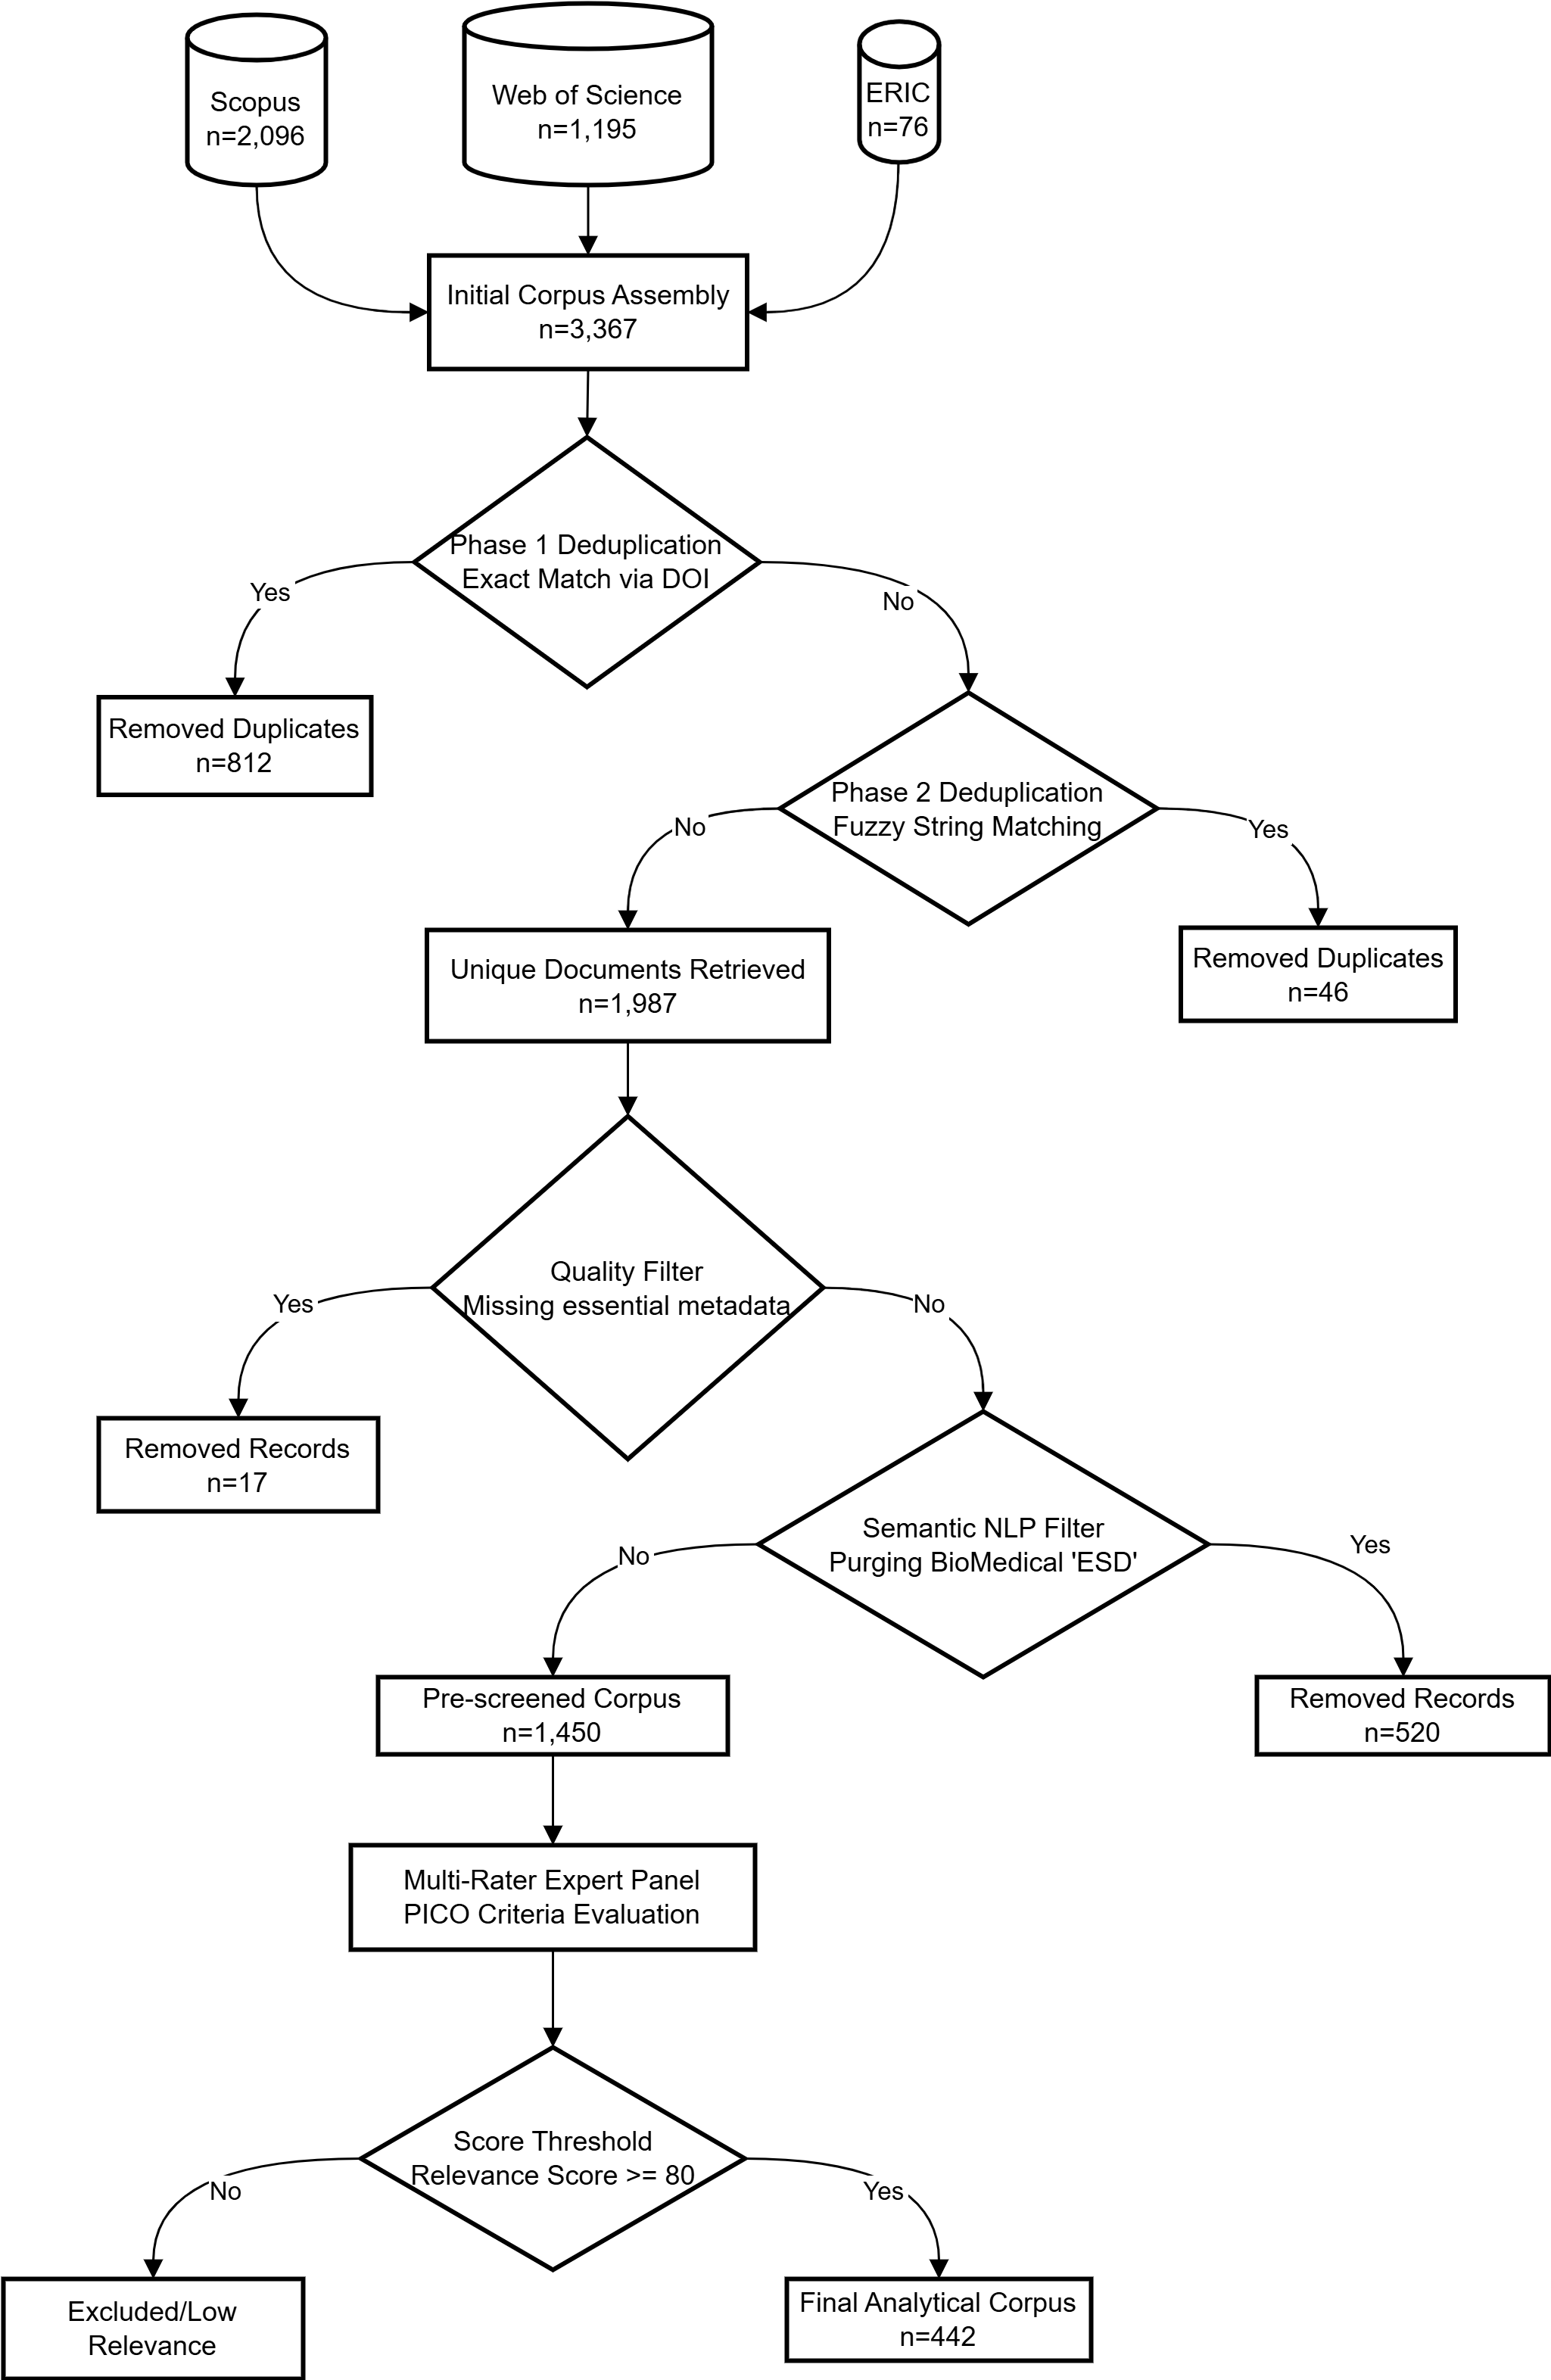
\includegraphics[width=0.45\textwidth]{enriquecimientoDataConsolidatinScreeningFlow.png}
	\caption{Data acquisition, deduplication, and screening flow. Three-database retrieval ($n = 3{,}367$) through sequential deduplication (DOI and fuzzy matching), quality filtering, semantic NLP screening, and PICO-based relevance evaluation, yielding the final analytical corpus ($n = 442$).}
	\label{fig:screening}
\end{figure}

Subsequently, records lacking essential metadata were eliminated ($n = 17$), and a natural language processing filter purged 520 biomedical entries erroneously indexed under the polysemic acronym ``ESD'' (Endoscopic Submucosal Dissection), yielding a pre-screened corpus of 1,450 documents.

A final relevance screening was conducted through a multi-rater expert panel applying PICO-adapted criteria (Population: higher education or vocational learners; Intervention: ESD-related pedagogical, curricular, or institutional actions; Context: tertiary or vocational settings; Outcome: sustainability competencies, literacy, or institutional transformation). Each document received a composite relevance score; only those achieving a threshold of 80 or above were retained. This stage crystallized the final analytical corpus of 446 highly relevant, metadata-complete documents (100\% abstract and title availability; 92.9\% DOI completeness).

\subsection{Science Mapping and Bibliometric Analysis}
\label{sec:analisis_bib}

The macroscopic architecture of the corpus was evaluated through science mapping methodologies designed to elucidate both the social networks of knowledge production and the latent cognitive structures governing the discipline \cite{mazov_methodological_2020, wang_research_2020}. Descriptive statistics were first generated to map publication trajectories, annual growth rates, and the most prolific actors---authors, institutions, and countries. Relational analyses then employed keyword co-occurrence to identify underlying epistemic themes \cite{callon_translations_1983, torcatoru_literature_2022}, bibliographic coupling to measure document similarity through shared references and detect invisible colleges \cite{kessler_bibliographic_1963, karimi_review_2025}, and reference co-citation to uncover the intellectual pillars of the field \cite{yildiz_examining_2019, ali_performance_2019}. Network visualizations were generated using VOSviewer, with temporal overlays permitting the differentiation between consolidated conceptual areas and nascent research frontiers. A state-of-the-art knowledge gap analysis further examined methods-by-concepts coverage matrices to systematically identify structural, declared, and emergent gaps across the corpus.

\subsection{Artificial Intelligence-Assisted Inductive Thematic Analysis}
\label{sec:sintesis_metodo}

To transcend the macroscopic limitations of network analysis and capture the qualitative depth embedded within the substantive text, this review incorporated a Large Language Model-assisted inductive thematic analysis \cite{moia_llm_2026, wen_leveraging_2026}. The 446 abstracts were processed through two complementary architectures: Qwen3-235B for thematic extraction and DeepSeek V3.2 for cross-thematic reasoning. The deployment of generative AI in qualitative synthesis represents an emergent paradigm that significantly augments analytical capacity while demanding strict methodological oversight \cite{lopez-pineda_validation_2025, ramirez-correa_mapping_2026}.

The analysis proceeded through a three-phase inductive pipeline (Figure~\ref{fig:thematic_clusters}). In Phase 1 (Inductive Thematic Mapping), the corpus was processed in 15 analytic batches to identify and define emergent conceptual categories without the imposition of \textit{a priori} theoretical frameworks. This iterative process yielded five primary thematic clusters characterizing the current discourse. In Phase 2 (Cross-Thematic Analysis), the system analyzed the latent structural relationships binding these themes, surfacing dominant analytical axes that delineate the field's organizing tensions. In Phase 3 (Framework Construction), the synthesized axes were utilized to construct integrative frameworks linking institutional, pedagogical, and outcome dimensions.

\begin{figure}[htbp]
	\centering
	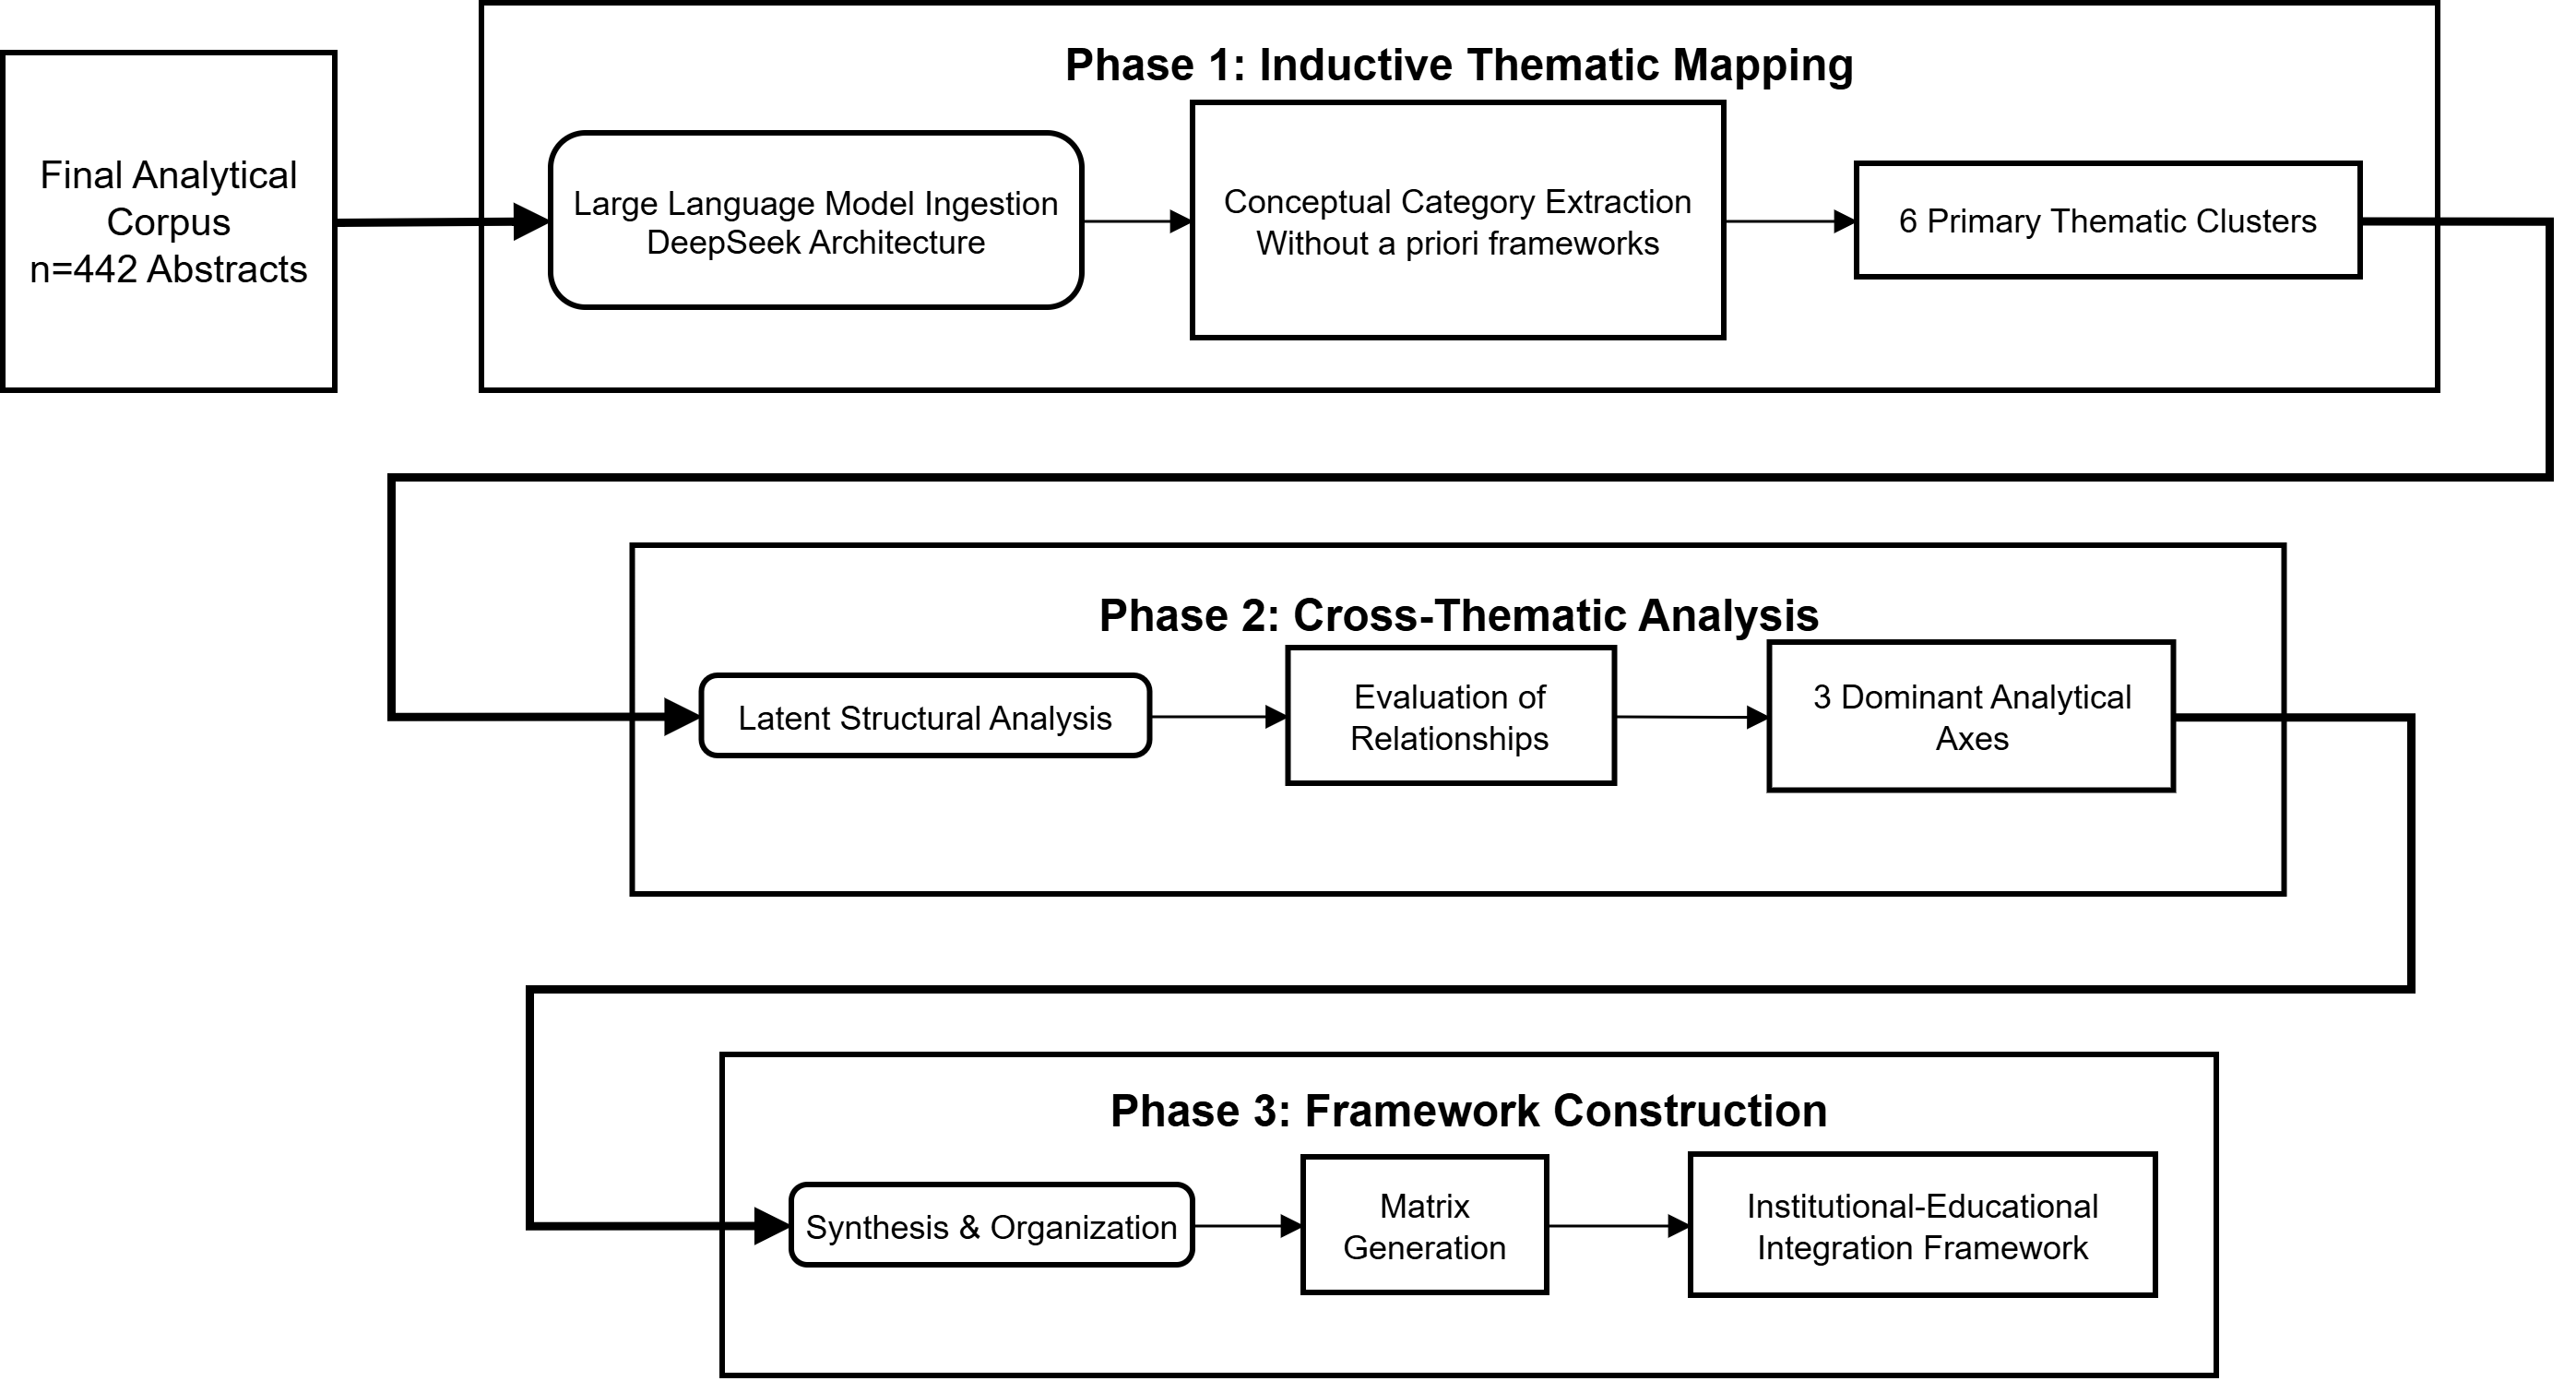
\includegraphics[width=0.65\textwidth]{TemasInductivos.png}
	\caption{Three-phase inductive thematic analysis pipeline. Phase 1: Large Language Model ingestion and emergent category extraction (5 thematic clusters). Phase 2: Latent structural analysis and cross-thematic relationship evaluation. Phase 3: Analytical framework construction.}
	\label{fig:thematic_clusters}
\end{figure}

To rigorously mitigate the inherent risks of stochastic algorithmic hallucination \cite{luna_chontal_task_2026}, a stringent verification protocol was embedded into the pipeline (Figure~\ref{fig:triangulation_protocol_new}). The platform computationally verified thematic propositions directly against the original source text of the abstracts, yielding a Grounding Score of 97\%. A total of 15 hallucination flags were identified and manually reviewed; all instances were critically validated or corrected by the research team to ensure the fidelity of the qualitative synthesis.

\begin{figure}[htbp]
	\centering
	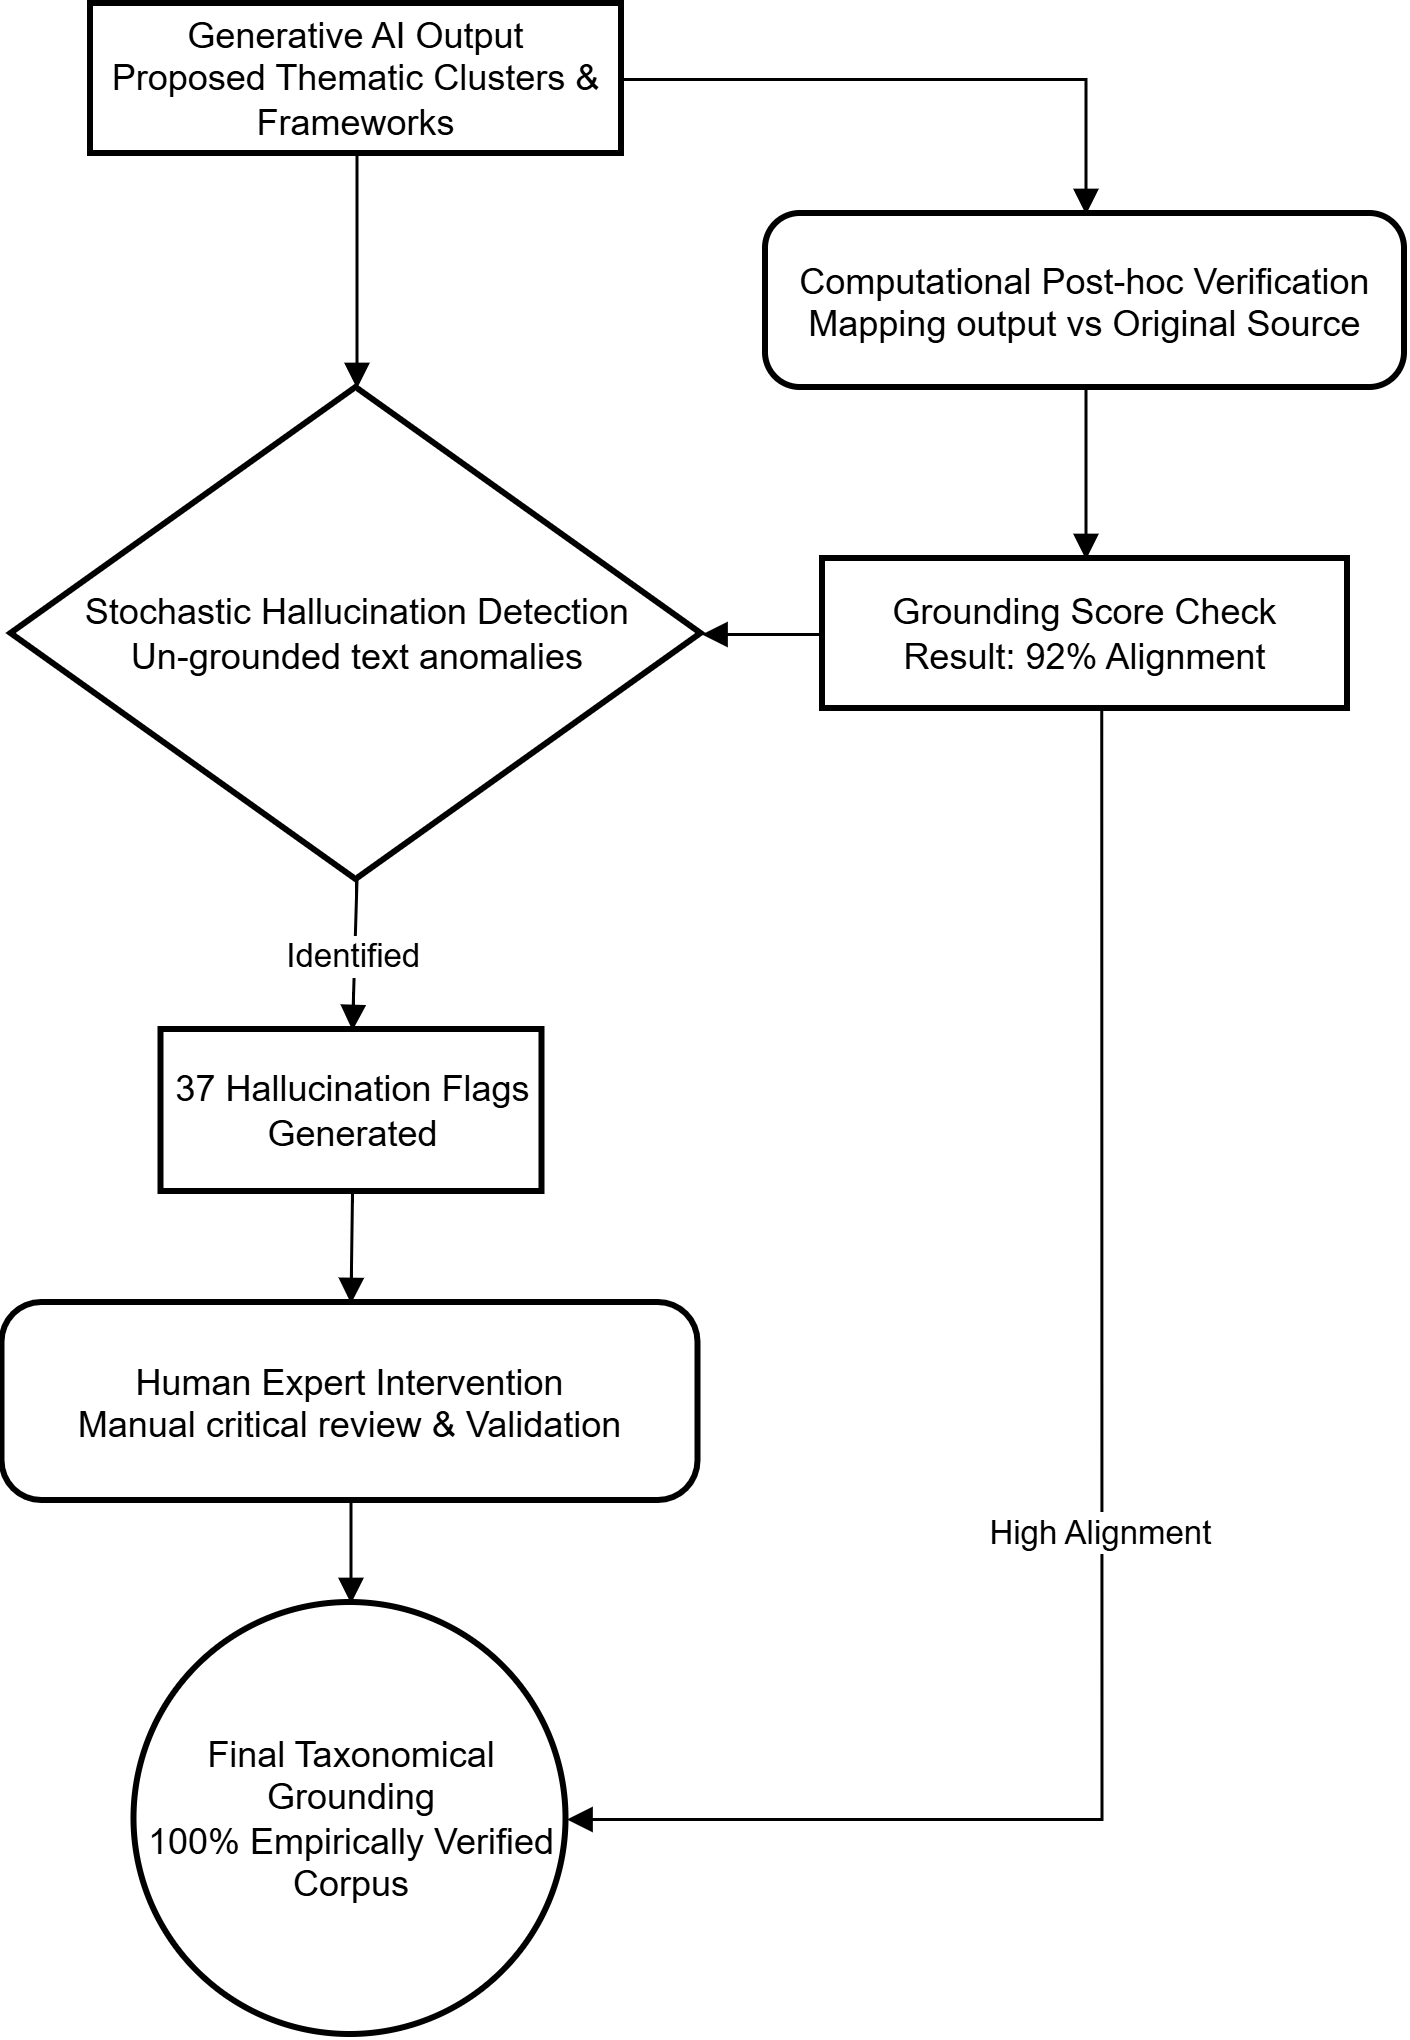
\includegraphics[width=0.45\textwidth]{traingaulacionVerificacion.png}
	\caption{Hallucination control and verification protocol. Computational post-hoc verification of AI-generated thematic outputs against original source abstracts, yielding a 97\% Grounding Score with 15 hallucination flags submitted to human expert review.}
	\label{fig:triangulation_protocol_new}
\end{figure}

% =============================================================================
% RESULTS
% =============================================================================

\section{Results}
\label{sec:resultados}

\subsection{Descriptive Profile and Temporal Dynamics of the Corpus}

The systematic search yielded a final corpus of 446 documents spanning the period 2015--2026. The temporal distribution reveals a marked acceleration in scholarly output that can be segmented into three distinct phases (Figure~\ref{fig:temporal}). During the initial phase (2015--2018), production remained modest but grew steadily, with 33 documents in 2015--2016 and 50 in 2017--2018, reflecting an early consolidation of the field following the adoption of the 2030 Agenda. The intermediate phase (2019--2022) witnessed substantial growth, from 65 documents in 2019--2020 to 71 in 2021--2022, coinciding with the publication of UNESCO's \textit{ESD for 2030 Roadmap} and the global mobilization around SDG 4.7. The acceleration phase (2023--2026) confirms exponential expansion, with 121 documents in 2023--2024 and 106 already registered for 2025--2026---the latter figure being provisional given ongoing indexation. The single most productive year is 2025, with 90 documents, underscoring the field's continued momentum. Overall, the corpus exhibits a compound annual growth rate that accelerated notably after 2019, with a relative research interest index rising from 0.049 in 2015 to 0.202 in 2025.

\begin{figure}[htbp]
	\centering
	
\includegraphics[width=\textwidth]{temporal_trends.png}
	\caption{Annual scientific production in the corpus ($n = 446$, 2015--2026).}
	\label{fig:temporal}
\end{figure}

The citation landscape is anchored by a small number of foundational publications that have accumulated disproportionate influence. The corpus accrued 10,332 total citations, yielding a mean of 23.17 citations per document and an h-index of 48. Table~\ref{tab:most_cited} presents the ten most-cited documents, which collectively define the field's empirical and conceptual foundations. Notably, \cite{filho_future_2015} leads with 646 citations, followed by \cite{boldureanu_entrepreneurship_2020} with 590 and \cite{cebrian_competencies_2015} with 454. The temporal distribution of these landmark works is revealing: the period 2015--2020 contributes all ten entries, with 2015 and 2020 each providing three---a pattern that reflects the convergence of foundational handbooks and SDG implementation frameworks during this period.

\begin{table}[htbp]
\centering
\caption{Ten most-cited documents in the corpus}\label{tab:most_cited}

\begin{tabular*}{\textwidth}{p{0.8cm}p{2.5cm}p{3.5cm}p{2.8cm}r}
\toprule
\textbf{Rank} & \textbf{Document} & \textbf{Title (abbreviated)} & \textbf{Journal} & \textbf{Citations} \\
\midrule
1 & \cite{filho_future_2015} & The future we want: Key issues on SD in HE & \textit{Int. J. Sustain. High. Educ.} & 646 \\
2 & \cite{boldureanu_entrepreneurship_2020} & Entrepreneurship education through successful models in HEIs & \textit{Sustainability} & 590 \\
3 & \cite{cebrian_competencies_2015} & Competencies in ESD: student teachers' views & \textit{Sustainability} & 454 \\
4 & \cite{barth_routledge_2015} & Routledge Handbook of HE for SD & \textit{Routledge} & 406 \\
5 & \cite{b_franco_higher_2019} & Higher education for SD: actioning the global goals & \textit{Sustainability Science} & 298 \\
6 & \cite{filho_identifying_2017} & Identifying and overcoming obstacles to SD at universities & \textit{J. Integr. Environ. Sci.} & 268 \\
7 & \cite{albareda-tiana_implementing_2018} & Implementing the SDGs at university level & \textit{Int. J. Sustain. High. Educ.} & 258 \\
8 & \cite{filho_sustainability_2020} & Sustainability leadership in HEIs: challenges & \textit{Sustainability} & 254 \\
9 & \cite{ferguson_sdg_2020} & SDG 4 in higher education: challenges and opportunities & \textit{Int. J. Sustain. High. Educ.} & 211 \\
10 & \cite{al-naqbi_status_2018} & Status of ESD and sustainability knowledge in UAE & \textit{Int. J. Sustain. High. Educ.} & 188 \\
\botrule
\end{tabular*}
\begin{tablenotes}
\item Citation counts retrieved from Scopus/WoS at the time of analysis.
\end{tablenotes}
\end{table}

\subsection{Geographic, Institutional, and Disciplinary Distribution}

The geographic analysis reveals a predominantly European concentration, with Spain leading the corpus ($n = 63$ articles, 14.1\%), followed by the United Kingdom ($n = 52$, 11.7\%) and Germany ($n = 40$, 9.0\%). The United States ($n = 27$, 6.1\%) and Brazil ($n = 17$, 3.8\%) represent the strongest non-European contributions, while Portugal ($n = 16$), South Africa and Sweden ($n = 14$ each), Italy ($n = 13$), and Colombia ($n = 12$) complete the top ten. The dominance of Iberian and Germanic countries, combined with meaningful Latin American and African participation, delineates a field whose intellectual center of gravity resides in Western Europe but with increasingly diversified global engagement. Eighty-six countries and 526 institutions are represented across the corpus, confirming the transnational character of ESD research.

The co-authorship network by countries (Figure~\ref{fig:coauth_countries}) identifies 86 nations organized into 15 clusters. The United Kingdom occupies the most connected position with 30 co-authorship links and a total link strength (TLS) of 55, functioning as the primary hub for international collaboration. Germany follows with 22 links (TLS = 39), maintaining strong ties to Spanish-speaking and Latin American partners. Spain ranks third in collaborative connectivity (19 links, TLS = 36) despite leading in absolute publication volume---a finding that underscores Spain's strength as a national producer rather than as an international broker. A notable Nordic--Gulf cluster emerges around Sweden, Denmark, Finland, and Qatar, while the Ibero-American cluster connects Spain, Colombia, Mexico, and Portugal through shared linguistic and institutional networks. Nine countries remain isolates with no co-authorship links, revealing persistent gaps in the field's global integration.

\begin{figure}[htbp]
	\centering
	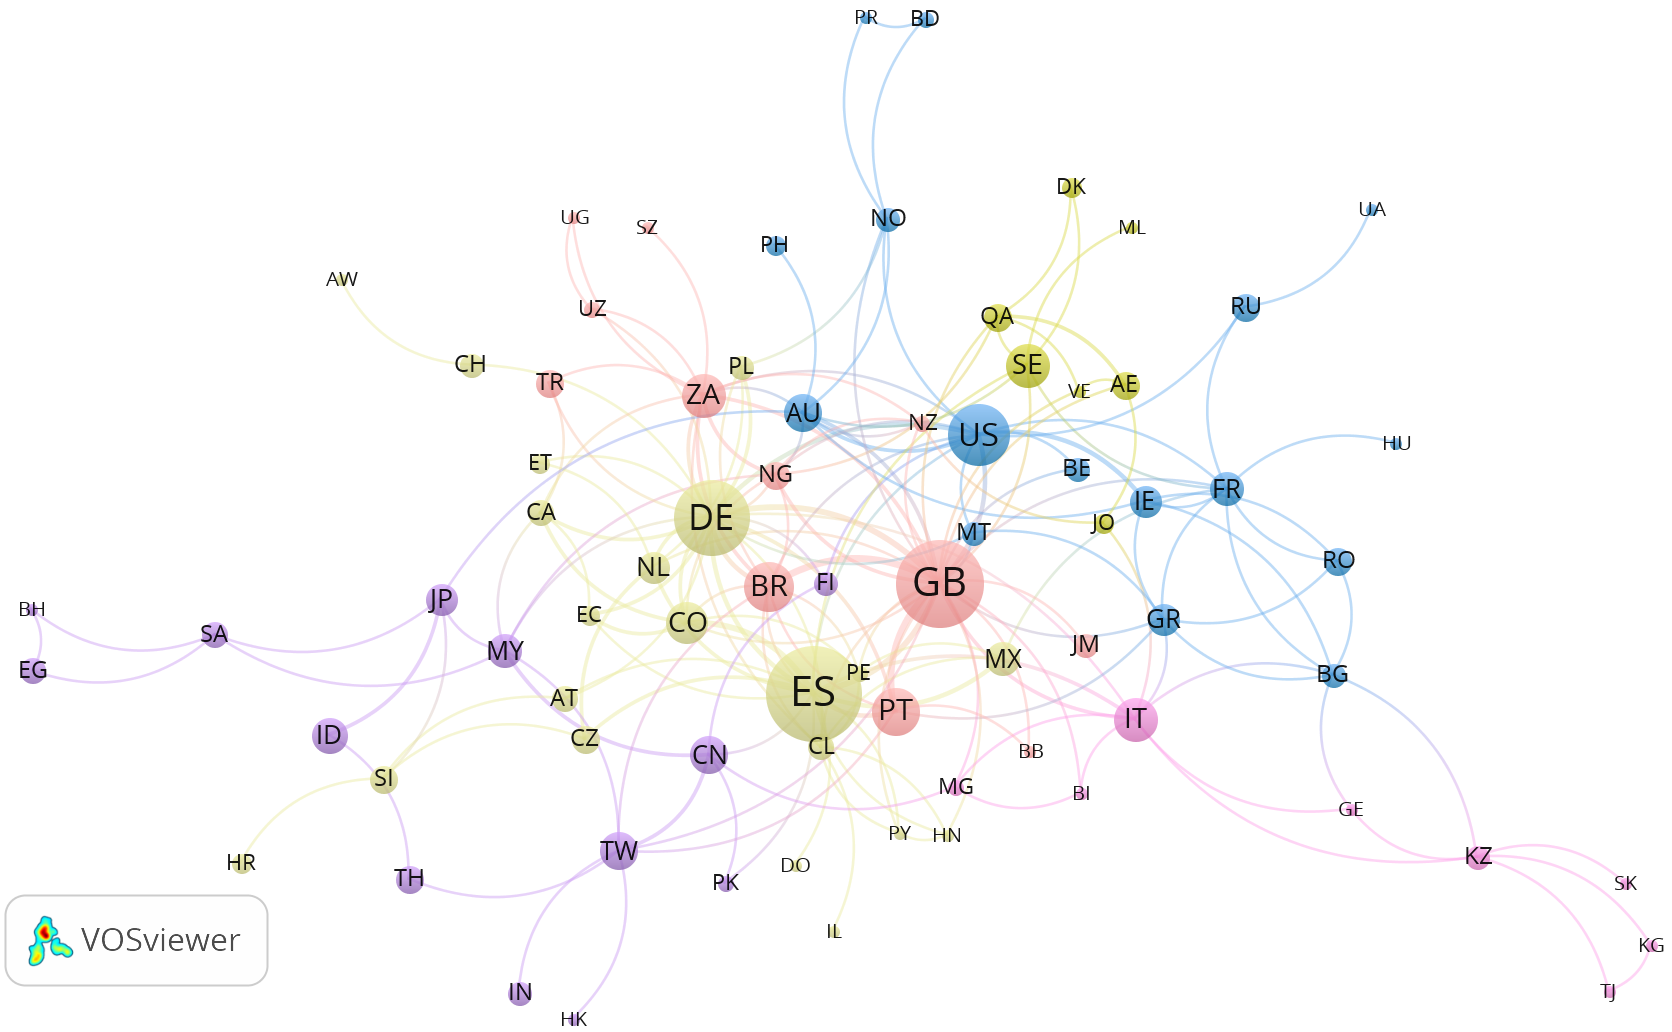
\includegraphics[width=\textwidth]{coauthorship_countries.png}
	\caption{Co-authorship network by countries (VOSviewer). Nodes sized by number of documents; colors indicate clusters; link thickness proportional to co-authorship strength. 86 nations, 15 clusters.}
	\label{fig:coauth_countries}
\end{figure}

The bibliographic coupling analysis at the institutional level reveals that the most intellectually interconnected institutions are Universit\"{a}t Hamburg (TLS = 2,812), Universidade Aberta (TLS = 2,375), Manchester Metropolitan University (TLS = 2,345), HAW Hamburg (TLS = 2,053), and Universidade Nova de Lisboa (TLS = 2,032). These institutions, organized into 41 clusters across 502 nodes, form distinct collaborative axes: a German sustainability science axis anchored by Hamburg institutions and Leuphana University of L\"{u}neburg (TLS = 1,517); a Portuguese--Brazilian network centered on Universidade Aberta, Universidade Nova de Lisboa, and Universidade Federal de Santa Maria; and a UK education cluster around Manchester Metropolitan University. Universidad de Salamanca (TLS = 1,508) bridges the Spanish-speaking network with the broader European core.

The disciplinary distribution, extracted from 137 unique discipline classifications, confirms the field's interdisciplinary character. Teacher Education leads ($n = 18$), followed by Engineering ($n = 12$), Business ($n = 11$), and Geography ($n = 9$), while early childhood education, environmental engineering, and science education contribute smaller but distinctive streams. The ratio of unique disciplines to total articles (137/446 = 0.31) indicates that nearly one-third of all articles self-identify within distinct disciplinary frameworks---a hallmark of a transdisciplinary field still negotiating its boundaries.

\subsection{Journal Landscape and Core Publication Venues}

The journal co-citation analysis identifies 1,150 sources organized into 105 clusters, revealing a highly differentiated yet hierarchically structured publication landscape. A clear two-journal dominance pattern emerges: the \textit{International Journal of Sustainability in Higher Education} (IJSHE) leads with a TLS of 4,240 and 230 co-citations, followed closely by \textit{Sustainability} (Switzerland) with a TLS of 3,979 and 200 co-citations. Notably, the \textit{Journal of Cleaner Production} ranks third (TLS = 3,960, 210 co-citations), occupying a nearly equivalent position that signals the field's strong connection to applied sustainability science. \textit{Environmental Education Research} (TLS = 2,837) and \textit{Sustainability Science} (TLS = 2,074) complete the top five. The bibliographic coupling of journals (161 journals, 31 clusters) corroborates this structure, with \textit{Sustainability} (TLS = 1,544) and IJSHE (TLS = 1,464) jointly anchoring the core cluster (Table~\ref{tab:journals}).

\begin{table}[htbp]
\centering
\caption{Top ten journals by co-citation frequency in the network}\label{tab:journals}
\begin{tabular*}{\textwidth}{@{\extracolsep\fill}clrrc}
\toprule
\textbf{Rank} & \textbf{Journal} & \textbf{Co-cit.} & \textbf{TLS} & \textbf{Cluster} \\
\midrule
1 & \textit{Int. J. Sustain. High. Educ.} & 230 & 4,240 & 1 \\
2 & \textit{J. Clean. Prod.} & 210 & 3,960 & 1 \\
3 & \textit{Sustainability (Switzerland)} & 200 & 3,979 & 20 \\
4 & \textit{Environ. Educ. Res.} & 150 & 2,837 & 4 \\
5 & \textit{Sustain. Sci.} & 113 & 2,074 & 1 \\
6 & \textit{J. Educ. Sustain. Dev.} & 90 & 1,412 & 1 \\
7 & \textit{World Sustain. Ser.} & 63 & 922 & 1 \\
8 & \textit{J. Environ. Educ.} & 51 & 827 & 4 \\
9 & \textit{Higher Education} & 48 & 781 & 11 \\
10 & \textit{Sustain. Dev.} & 44 & 737 & 1 \\
\botrule
\end{tabular*}
\begin{tablenotes}
\item TLS = total link strength in the co-citation network.
\end{tablenotes}
\end{table}

Three distinct cluster families warrant attention. Cluster 1 forms the core ESD--higher education nexus, anchoring IJSHE alongside \textit{Journal of Cleaner Production}, \textit{Sustainability Science}, and the \textit{World Sustainability Series}. Cluster 4 concentrates environmental and science education journals, including \textit{Environmental Education Research} and \textit{The Journal of Environmental Education}, reflecting the legacy of environmental education research that preceded and now intersects with ESD. Cluster 11, centered on \textit{Higher Education}, represents the higher education policy and governance interface.

\subsection{Intellectual Structure: Co-citation and Bibliographic Coupling Analysis}

The reference co-citation analysis identifies 1,067 cited references organized into 54 clusters, revealing the field's intellectual DNA. Wiek et al. (2011) emerges as the single most co-cited reference (TLS = 1,082; 66 co-citations), establishing key competencies in sustainability as the foundational framework for the entire field. This seminal reference anchors Cluster 3---the largest cluster with 241 nodes---which also encompasses Barth et al. (2007; TLS = 483), Sipos et al. (2008; TLS = 463), and Lozano et al. (2017; TLS = 356), collectively constituting the competence-framework tradition (Figure~\ref{fig:cocitation}). Lozano emerges as the most recurrent author in the co-citation network, with four distinct publications appearing among the ten most co-cited references (2006, 2011, 2014, 2017), spanning from institutional transformation to competence operationalization.

The co-citation structure reveals five intellectual pillars:

\begin{enumerate}
    \item \textbf{Competence frameworks and sustainability key competencies} (Cluster 3): Wiek et al. (2011), Barth et al. (2007), Sipos et al. (2008), Lozano et al. (2017), Brundiers et al. (2010, 2020), UNESCO (2017, 2020).
    \item \textbf{Institutional transformation and whole-institution approaches} (Cluster 2): Wals (2013; TLS = 356), Pauw et al. (2015), O'Flaherty and Liddy (2017).
    \item \textbf{Curriculum integration and ESD embedding} (Cluster 4): Lambrechts et al. (2012), Mula et al. (2017), Mochizuki and Fadeeva (2010), Bertschy et al. (2013).
    \item \textbf{Campus sustainability and assessment} (Cluster 5): Lozano (2011; TLS = 422), Lozano (2006; TLS = 300), Lozano (2014; TLS = 314).
    \item \textbf{Environmental behavior and attitudes} (Cluster 7): Kollmuss and Agyeman (2002), Shephard (2008), Kopnina (2014).
\end{enumerate}

\begin{figure}[htbp]
	\centering
	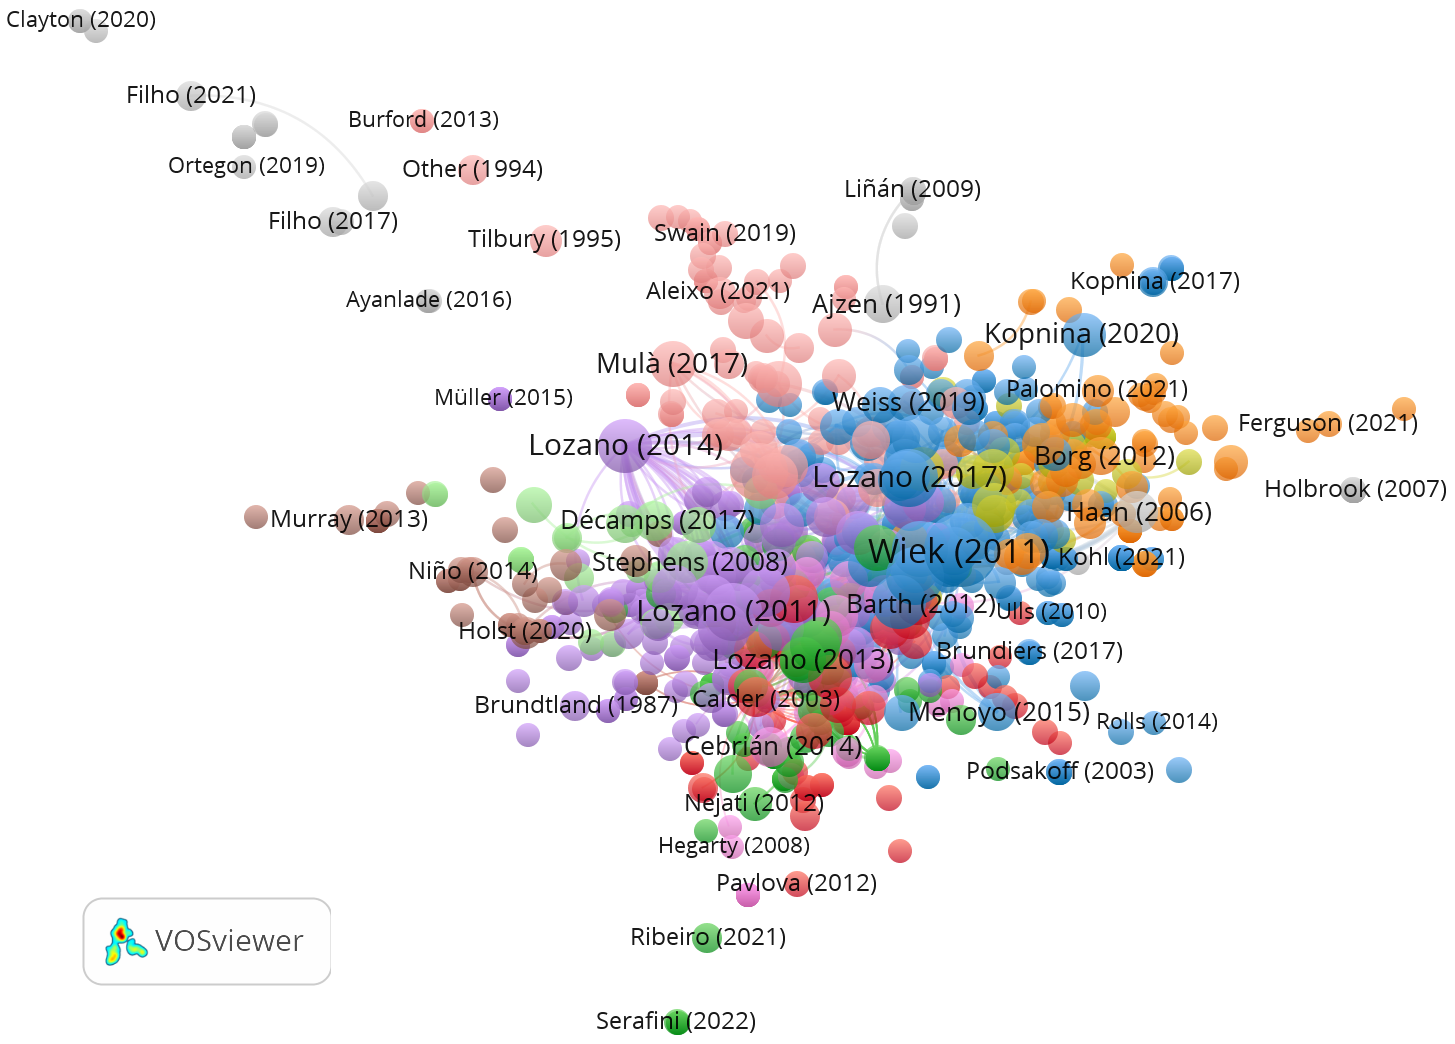
\includegraphics[width=\textwidth]{cocitation.png}
	\caption{Reference co-citation network (VOSviewer). Cluster visualization showing intellectual pillars. 1,067 references, 54 clusters. Node size proportional to co-citation frequency; colors indicate thematic clusters.}
	\label{fig:cocitation}
\end{figure}

Bibliographic coupling analysis of the 446 documents (369 of which met the minimum citation threshold) further corroborates this structure. The highest-coupled documents---\cite{albareda-tiana_implementing_2018} (TLS = 427), \cite{faham_using_2017} (TLS = 396), and Brandt et al. (2022; TLS = 351)---share extensive reference lists focused on competence orientation and SDG implementation. Critically, citation count and coupling strength do not always correlate: \cite{filho_future_2015}, the most-cited document (646 citations), exhibits relatively low coupling strength (TLS = 34), indicating that it is widely cited but draws on a reference base distinct from the field's mainstream. Conversely, \cite{disterheft_indicare-model_2016} (TLS = 350) and \cite{brassler_fostering_2021} (TLS = 348) occupy highly coupled positions despite moderate citation counts, suggesting their role as intellectual bridges within the network.

\subsection{Conceptual Structure: Keyword Co-occurrence Analysis}

The keyword co-occurrence network (Figure~\ref{fig:keyword_coocc}) encompasses 352 keywords organized into seven thematic clusters, offering a fine-grained map of the conceptual territory. The three most central keywords are \textit{sustainable development} (TLS = 1,204; 166 occurrences), \textit{higher education} (TLS = 833; 133 occurrences), and \textit{sustainability} (TLS = 705; 110 occurrences), followed by \textit{education for sustainable development} (TLS = 652; 131 occurrences). The strongest dyadic co-occurrence links---\textit{sustainable development}$\leftrightarrow$\textit{higher education} (weight = 63) and \textit{sustainable development}$\leftrightarrow$\textit{education for sustainable development} (weight = 58)---confirm that the field's conceptual nucleus remains firmly anchored in the ESD--higher education nexus.

\begin{figure}[htbp]
	\centering
	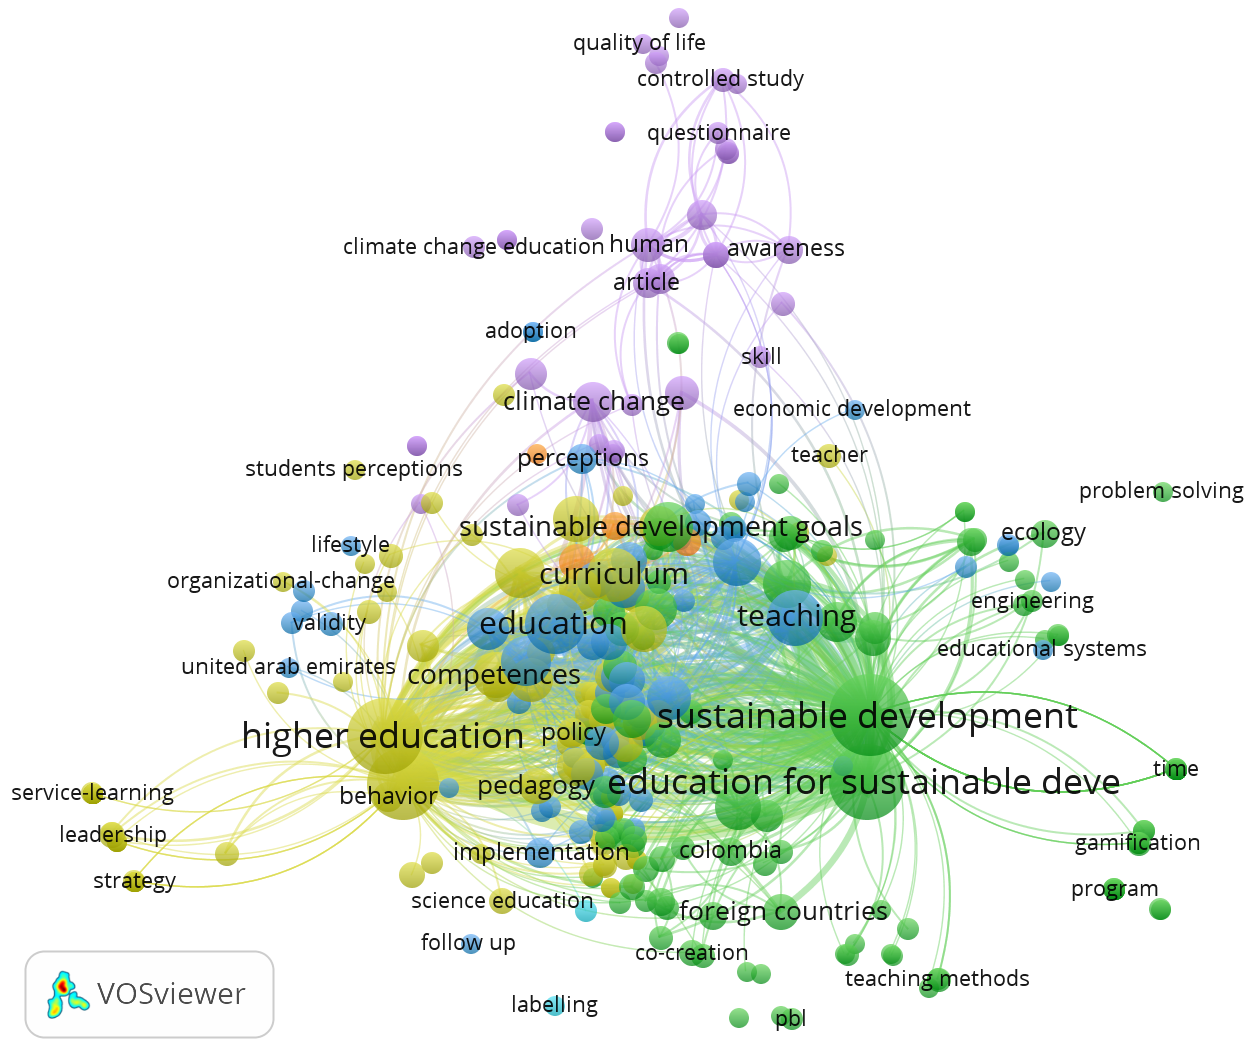
\includegraphics[width=\textwidth]{keyword_cooccurrence.png}
	\caption{Keyword co-occurrence network (VOSviewer). Cluster visualization of 352 keywords showing seven thematic clusters. Node size proportional to keyword frequency; link thickness proportional to co-occurrence strength.}
	\label{fig:keyword_coocc}
\end{figure}

Seven clusters delineate distinct yet interconnected conceptual territories:

\textbf{Cluster 1 (Sustainability -- Higher Education -- Curriculum)} revolves around \textit{sustainability}, \textit{higher education}, and \textit{curriculum}, capturing the normative and structural dimensions of sustainability integration. Keywords such as \textit{key competences}, \textit{systems thinking}, and \textit{experiential learning} indicate the operationalization of competence frameworks into curricular practice.

\textbf{Cluster 2 (ESD Implementation and SDG Alignment)} centers on \textit{education for sustainable development}, \textit{sustainable development goals}, and \textit{sustainable development}, incorporating \textit{transformative learning}, \textit{service learning}, and \textit{design thinking}. This is the largest cluster (124 nodes), capturing the implementation-oriented research that connects policy frameworks to pedagogical practice.

\textbf{Cluster 3 (Education, Teaching, and Student Behavior)} features \textit{education}, \textit{teaching}, \textit{learning}, \textit{knowledge}, \textit{attitudes}, and \textit{behavior}, constituting the core behavioral research cluster. This cluster captures the empirical tradition of measuring student-level outcomes through surveys and attitudinal instruments \cite{badea_impact_2020, alvarez-garcia_variables_2019}.

\textbf{Cluster 4 (Climate Change and Health Education)} is anchored by \textit{climate change} and \textit{climate change education}, with a mean publication year of approximately 2023---the most recent cluster average. The inclusion of nursing-related keywords reveals a discipline-specific pathway for climate literacy that bridges health and environmental education \cite{alvarez-nieto_developing_2018, bishr_effectiveness_2026}.

\textbf{Cluster 5 (Engineering, Interdisciplinarity, and Digital Learning)} unites \textit{curricula}, \textit{engineering education}, \textit{e-learning}, \textit{project-based learning}, and \textit{interdisciplinarity}, reflecting the technologically mediated strand of ESD research. The presence of \textit{circular economy} and \textit{massive open online course} keywords reveals emerging conceptual intersections.

\textbf{Cluster 7 (Vocational Education and Green Skills)} contains only four nodes but occupies a strategically important bridging position connecting vocational training with the ESD implementation cluster. The keyword \textit{green skills} signals its conceptual proximity to the growing workforce readiness agenda \cite{carstensen_mapping_2025, da_costa_addressing_2025}.

The density visualization reveals that the highest-density area concentrates around the \textit{sustainable development}--\textit{higher education}--\textit{education for sustainable development} triangle, while lower-density peripheral areas include \textit{climate change education}, \textit{vocational education}, \textit{green skills}, and \textit{circular economy}---terms that, while growing rapidly, remain underrepresented relative to the ESD core.

\subsection{Social Structure: Collaboration Patterns}

The co-authorship network by authors reveals a characteristic pattern of fragmented collaboration: research teams are predominantly small and largely independent, with no single dominant team spanning the entire field. The institutional co-authorship network (526 nodes, 200 clusters) exhibits extreme fragmentation, with an average cluster size of only 2.6 nodes and 107 institutions (20.3\%) remaining as isolates with no co-authorship links. The largest co-authorship cluster centers on Portuguese, Brazilian, and German universities---Universidade Aberta, Universit\"{a}t Hamburg, HAW Hamburg, and Manchester Metropolitan University---reflecting a Lusophone--Germanic collaborative axis \cite{caeiro_sustainability_2020, filho_sustainability_2020}. A German sustainability education cluster connects Leuphana University with Eberswalde University for Sustainable Development, while a Spanish--Latin American cluster bridges Universidad de Salamanca with Colombian and Mexican institutions.

This fragmented collaboration structure, while indicative of a diverse and distributed research community, also signals limited cross-regional and cross-paradigmatic exchange---a structural feature that may partially explain the conceptual fragmentation between ESD, climate literacy, and green skills traditions identified in the keyword analysis.

\subsection{Population, Methodological, and Instrumental Characterization}

The population analysis ($n = 446$ articles) reveals that students constitute the dominant study population. Aggregating all student-related categories---undergraduate students ($n = 43$, 9.6\%), university students ($n = 58$, 13.0\%), higher education students ($n = 28$, 6.3\%), business students ($n = 9$, 2.0\%), and engineering students ($n = 8$, 1.8\%)---yields approximately 146 articles (32.7\%) focused on the student experience. Articles classified under the broader category of ``Higher Education Context'' account for 73 (16.4\%), typically describing institutional settings without specifying a discrete study population. Faculty and educator categories collectively account for 31 articles (7.0\%), comprising university educators ($n = 13$), university faculty ($n = 12$), and teacher educators ($n = 6$). Pre-service teachers represent a distinctive population ($n = 21$, 4.7\%), bridging the student and educator domains (Table~\ref{tab:populations}).

\begin{table}[htbp]
\centering
\caption{Population categories distribution (top 10)}\label{tab:populations}
\begin{tabular}{l c c}
\toprule
\textbf{Population category} & $\boldsymbol{n}$ & \textbf{\%} \\
\midrule
Higher Education Context & 73 & 16.4 \\
University Students & 58 & 13.0 \\
Undergraduate Students & 43 & 9.6 \\
Higher Education Students & 28 & 6.3 \\
Pre-service Teachers & 21 & 4.7 \\
University Educators & 13 & 2.9 \\
University Faculty & 12 & 2.7 \\
Business Students & 9 & 2.0 \\
Higher Education Institutions & 9 & 2.0 \\
Engineering Students & 8 & 1.8 \\
\botrule
\end{tabular}
\end{table}

Research designs exhibit a similarly concentrated pattern. Survey designs lead ($n = 87$, 19.5\%), followed by case studies ($n = 81$, 18.2\%), qualitative approaches ($n = 50$, 11.2\%), and quantitative studies ($n = 43$, 9.6\%). Mixed-methods designs account for 30 articles (6.7\%), while interview-based studies contribute 26 (5.8\%). Experimental and quasi-experimental designs together account for only 18 articles (4.0\%), reflecting the field's limited engagement with controlled interventional research---a critical gap for establishing causal evidence on pedagogical effectiveness. Content analysis ($n = 23$) and systematic reviews ($n = 13$) represent the documentary and meta-analytic traditions, respectively (Table~\ref{tab:research_design}).

\begin{table}[htbp]
\centering
\caption{Research design distribution}\label{tab:research_design}
\begin{tabular}{l c c}
\toprule
\textbf{Research design} & $\boldsymbol{n}$ & \textbf{\%} \\
\midrule
Survey & 87 & 19.5 \\
Case Study & 81 & 18.2 \\
Qualitative & 50 & 11.2 \\
Quantitative & 43 & 9.6 \\
Mixed Methods & 30 & 6.7 \\
Interview-based & 26 & 5.8 \\
Content Analysis & 23 & 5.2 \\
Action Research & 15 & 3.4 \\
Experimental & 14 & 3.1 \\
Systematic Review & 13 & 2.9 \\
Quasi-experimental & 4 & 0.9 \\
\botrule
\end{tabular}
\end{table}

Among reported sample sizes ($n = 139$ studies, 31.2\% of the corpus), the median was 203 and the mean 1,576.2, with a range from 5 to 90,000. The pronounced right skew (mean/median ratio = 7.8:1) indicates that the evidence base is dominated by small-to-medium-scale studies, with a small number of large-scale surveys inflating the mean.

The research focus distribution (Table~\ref{tab:research_focus}) reveals that Curriculum Design and Integration ($n = 81$) leads the scholarly agenda, followed by Institutional Policy and Strategy ($n = 53$), Teaching Methods and Pedagogy ($n = 45$), and Framework and Model Development ($n = 40$). Professional Development ($n = 36$) and Learning Outcomes and Effectiveness ($n = 31$) form a second tier. The emergence of Review and Bibliometric Analysis as a distinct focus ($n = 31$) reflects the field's growing reflexive awareness. Critically underrepresented areas include Technology and Digital Learning ($n = 13$) and Interdisciplinary and Systems Thinking ($n = 5$).

\begin{table}[htbp]
\centering
\caption{Research focus distribution}\label{tab:research_focus}
\begin{tabular}{l c c}
\toprule
\textbf{Research focus} & $\boldsymbol{n}$ & \textbf{\%} \\
\midrule
Curriculum Design \& Integration & 81 & 18.2 \\
Institutional Policy \& Strategy & 53 & 11.9 \\
Teaching Methods \& Pedagogy & 45 & 10.1 \\
Framework \& Model Development & 40 & 9.0 \\
Professional Development & 36 & 8.1 \\
Learning Outcomes \& Effectiveness & 31 & 7.0 \\
Review \& Bibliometric Analysis & 31 & 7.0 \\
Competencies \& Skills & 26 & 5.8 \\
Assessment \& Evaluation & 24 & 5.4 \\
Student Perceptions \& Attitudes & 22 & 4.9 \\
\botrule
\end{tabular}
\end{table}

The most commonly employed instruments are questionnaires ($n = 61$) and surveys ($n = 38$), which together account for 99 articles---confirming the field's reliance on self-report instruments. Interviews constitute the third most frequent tool ($n = 28$), followed by content analysis ($n = 14$) and case studies ($n = 12$). Project-based learning stands as the most frequently documented pedagogical intervention ($n = 11$), as exemplified by \cite{fuertes_camacho_integrating_2019}, \cite{cottafava_education_2019}, and \cite{ariza_bringing_2023}.

\subsection{Inductive Thematic Synthesis}

The inductive thematic analysis of 446 abstracts, conducted through iterative coding across 15 analytic batches using large language model-assisted extraction with systematic hallucination control, yielded five consolidated themes (Table~\ref{tab:thematic_tax}). The overall grounding score was 97\%, indicating high fidelity between extracted themes and source abstracts.

\begin{table}[htbp]
\centering
\caption{Consolidated thematic taxonomy}\label{tab:thematic_tax}
\begin{tabular*}{\textwidth}{p{4cm}p{6.5cm}p{1cm}}
\toprule
\textbf{Theme} & \textbf{Sub-themes} & \textbf{Robustness} \\
\midrule
1. ESD Integration in Curricula & (a) Curriculum reform and subject-specific integration; (b) Barriers to ESD implementation & High \\ \addlinespace
2. Transformative Pedagogies and Experiential Learning & (a) Student engagement through experiential learning; (b) Transformative and transdisciplinary pedagogies & High \\ \addlinespace
3. Institutional and Faculty Roles in Advancing ESD & (a) Faculty and institutional leadership; (b) Educator transformation and professional development & High \\ \addlinespace
4. Sustainability Literacy, Values, and Behavioral Outcomes & (a) Sustainability literacy and assessment; (b) Value-based learning and pro-environmental behavior & High \\ \addlinespace
5. Digital Innovation in ESD Delivery & (a) Digital and virtual learning environments; (b) Emerging technologies in sustainability education & High \\
\botrule
\end{tabular*}
\end{table}

Theme 1 (ESD Integration) captures studies focused on embedding sustainability principles into curricular structures, including SDG alignment \cite{ahmad_codesigns_2023, balan_connecting_2025} and the persistent challenges of institutional resistance and faculty awareness gaps \cite{acosta-castellanos_education_2022}. Theme 2 (Transformative Pedagogies) spans active learning strategies such as project-based learning \cite{du_university_2022}, experiential approaches including service learning and community engagement \cite{alvarez-vanegas_empowering_2024}, and technology-mediated instruction encompassing serious games \cite{cravero_learning_2021} and augmented reality \cite{czok_learning_2023}. Theme 3 (Institutional Roles) documents the enabling conditions for curricular transformation, finding that teacher training programs precede and facilitate institutional change \cite{biasutti_educating_2018}. Theme 4 (Sustainability Literacy) addresses the acquisition of knowledge, attitudes, behaviors, and values as educational outcomes, measured through instruments such as sustainability literacy tests and pre--post evaluations. Theme 5 (Digital Innovation), the most temporally recent, reflects the growing role of virtual reality, digital twins, artificial intelligence, and online academies in ESD delivery.

The cross-analysis identified three recurring inter-thematic configurations: (1) an \textbf{Integrated Education Design} configuration linking curriculum, pedagogy, and competencies as a coherent teaching--learning system; (2) an \textbf{Institutional Support System} linking organizational strategies with educator development as enabling conditions; and (3) a \textbf{Technology-Enhanced Learning} trajectory connecting digital innovation with both pedagogical approaches and student outcomes.

\subsection{Research Frontiers and Knowledge Gaps}

The state-of-the-art analysis identified 56 knowledge gaps classified into three taxonomic categories: structural gaps ($n = 25$), declared gaps ($n = 23$), and emergent gaps ($n = 8$). The coverage analysis of Methods $\times$ Concepts matrices revealed 64.0\% coverage (48 of 75 cells populated), while Methods $\times$ Applications achieved 74.1\% coverage, indicating that approximately one-third of methodologically plausible combinations remain unexplored.

\textbf{Structural gaps} represent combinations of frequent approaches and domains that never co-occur in the corpus. The qualitative research tradition accounts for multiple structural gaps, being systematically absent from biology, clinical, and medical domains---suggesting that human-dimension research has not penetrated health and natural-science sustainability subfields. The simulation--pedagogy and case study--ecology gaps indicate that innovative methodological approaches have not been systematically paired with emerging content domains.

\textbf{Declared gaps}, explicitly articulated by researchers within their abstracts, reveal a convergent pattern of concerns (Table~\ref{tab:knowledge_gaps}). Multiple studies note the scarcity of longitudinal research on ESD intervention effects \cite{brassler_interdisciplinary_2025, collado_innovation_2022}, the limited investigation of comparative studies between training formats \cite{brassler_students_2021}, and the absence of causal models of sustainability competency acquisition \cite{abdullahi_impact_2024}. Researchers also identify insufficient attention to ESG integration in general education \cite{chien_evaluating_2025} and the need for mixed-method approaches to capture institutional change dynamics \cite{da_costa_addressing_2025}.

\begin{table}[htbp]
\centering
\caption{Selected declared knowledge gaps with representative references}\label{tab:knowledge_gaps}
\begin{tabular*}{\textwidth}{@{\extracolsep\fill}p{0.45\textwidth}p{0.45\textwidth}}
\toprule
\textbf{Gap area} & \textbf{Key references} \\
\midrule
Longitudinal impact assessment of ESD interventions & \cite{brassler_interdisciplinary_2025}; \cite{collado_innovation_2022} \\
Comparison between ESD delivery formats & \cite{brassler_students_2021} \\
Causal models of sustainability competency acquisition & \cite{abdullahi_impact_2024} \\
ESG and financial sustainability in curricula & \cite{chien_evaluating_2025}; \cite{garcia-hernandez_structural_2025} \\
Scalability across geographic and institutional contexts & \cite{alvarez-vanegas_empowering_2024} \\
Mixed-method approaches for institutional change & \cite{da_costa_addressing_2025} \\
\botrule
\end{tabular*}
\end{table}

\textbf{Emergent gaps} arise from rapidly growing areas that lack adequate methodological coverage. Simulation-based approaches show the highest growth rate (new entrant with 8 uncovered combinations), yet remain disconnected from pedagogical theory. Quantitative methods (2.36$\times$ growth) have seven uncovered combinations with key domains, while medical (2.81$\times$ growth) and clinical applications (2.11$\times$ growth) present expanding frontiers with insufficient qualitative coverage. The fastest-growing research frontiers include simulation (new), economic growth (3.37$\times$), medical applications (2.81$\times$), pedagogy as a concept (2.39$\times$), and quantitative methods (2.36$\times$).

\begin{figure}[htbp]
	\centering
	
\includegraphics[width=\textwidth]{coverage_methods_concepts.png}
	\caption{Methods $\times$ Concepts coverage matrix (64.0\% coverage). Empty cells indicate structural knowledge gaps.}
	\label{fig:coverage}
\end{figure}

The convergence of these findings points to a field in active conceptual transition. The traditional ESD paradigm---rooted in competence frameworks, institutional transformation, and curriculum integration---is progressively intersecting with climate-specific constructs (climate literacy, climate action competence), green economy demands (green skills, sustainable entrepreneurship; \cite{garcia-hernandez_structural_2025}; \cite{carstensen_mapping_2025}), and digitally mediated pedagogies (simulations, serious games, AI-enhanced learning). Yet the evidence base remains characterized by survey and case-study dominance, limited experimental rigor, geographic Euro-centrism, and fragmented collaboration networks. The structural absence of qualitative research from health and natural-science domains and the emergent but methodologically underdeveloped frontiers of simulation and digital learning constitute the most pressing gaps for the next generation of ESD research in higher education and vocational education contexts.

% =============================================================================
% DISCUSSION
% =============================================================================

\section{Discussion}
\label{sec:discusion}

The bibliometric mapping and inductive thematic analysis of 446 documents spanning 2015--2026 reveal that Education for Sustainable Development (ESD) in higher education is no longer a peripheral curricular concern but has become a structurally consolidated research field with identifiable intellectual pillars, persistent geographic asymmetries, and critical methodological blind spots. Five emergent themes---curriculum integration, transformative pedagogies, institutional and faculty roles, sustainability literacy and behavioral outcomes, and digital innovation---collectively delineate a field whose conceptual nucleus remains anchored in the competence-framework tradition \cite{wiek_operationalising_2015} yet is progressively intersecting with climate-specific constructs and green economy demands. Rather than reiterating descriptive metrics, this discussion interprets the latent tensions, structural imperatives, and emergent frontiers that these findings expose, drawing upon contemporary multidisciplinary evidence to bridge academic theory and global praxis.

\subsection{Aligning Educational Outcomes with the Green Economy: Geographic Asymmetries and Curricular Gaps}

The keyword co-occurrence analysis identified \textit{green skills} and \textit{circular economy} as rapidly growing yet peripheral concepts, occupying low-density areas in the network despite their increasing policy urgency. This finding signals a persistent misalignment between the field's conceptual core---still gravitating around generic sustainability competencies---and the concrete workforce demands of the green transition. As nations commit to aggressive decarbonization and circular economy models, higher education institutions (HEIs) are increasingly tasked with producing human capital fluent in green finance, sustainable industrialization, and climate adaptation strategies \cite{tamasiga_green_2025, desalegn_developing_2022}. Yet our results reveal that this pressure is unevenly distributed: Spain, the United Kingdom, and Germany collectively account for over one-third of all publications, while the Global South---with the notable exceptions of Brazil, South Africa, and Colombia---remains structurally underrepresented. This geographic concentration, corroborated by the co-authorship network where nine countries remain isolates with no collaborative links, underscores a systemic gap in current ESD paradigms. Developing nations face acute challenges in balancing rapid industrialization with environmental imperatives, necessitating localized, context-sensitive educational frameworks rather than imported models \cite{ndoka_comparative_2025, dias_paiao_junior_economic_2024}. Universities must transcend theoretical environmentalism to engage in economic diversification, equipping graduates with the analytical acumen to operationalize the SDGs within complex socioeconomic ecosystems \cite{st_flour_sustainability_2021}. The future of ESD must therefore be intrinsically linked to labor market realities, systematically translating academic sustainability into actionable green skills that drive industrial transformation and mitigate climate externalities \cite{garcia-hernandez_structural_2025}.

\subsection{Pedagogical Transformation, Sustainability Literacy, and the Measurement Challenge}

The dominance of Theme 2 (Transformative Pedagogies) and Theme 4 (Sustainability Literacy and Behavioral Outcomes) in our thematic synthesis confirms that the field has moved decisively beyond transmissive instruction toward experiential, student-centered paradigms. However, a critical tension emerges from the methodological characterization: surveys and case studies together account for nearly 38\% of all research designs, while experimental and quasi-experimental designs represent only 4.0\% of the corpus. This methodological imbalance constitutes a fundamental constraint on the field's capacity to establish causal evidence for pedagogical effectiveness. The literature consistently argues that complex ``wicked problems'' cannot be resolved within monodisciplinary silos, compelling HEIs to foster environments where students and external partners co-construct knowledge through authentic, real-world engagement \cite{kurris_facilitators_2026, leal_filho_promoting_2025}. SDG-aligned projects in STEM fields demonstrate that experiential learning significantly enhances interdisciplinary competencies, intercultural awareness, and intrinsic motivation \cite{poya_embedding_2026, roy_integrating_2025, johnson_comparisons_2026, hu_promoting_2026}. Embedding climate change adaptation into civil engineering curricula equips future professionals with both technical viability and ethical capacity for resilient infrastructure design \cite{dupuis_building_2025, kordi_teaching_2025, baah_building_2025}.

Yet the measurement of sustainability literacy---particularly the transition from ``knowing'' to ``doing''---remains a declared knowledge gap across the corpus. Our gap analysis identified the scarcity of longitudinal impact assessments and causal models of competency acquisition as the most recurrently articulated research needs. The concept of ``Work 5.0,'' combining human-centric principles with advanced technologies, demands a competence framework reliant on critical reflection, digital agility, and systems thinking \cite{zare_engineering_2026}. Contemporary ESD must therefore pivot from passive knowledge acquisition to radical identity transformation, cultivating agents of change who inherently view professional practice through the lens of planetary boundaries and social justice \cite{lopez_transformative_2025, ferreira_de_mello_classroom_2026}.

\subsection{The Institutional Architecture: From Declarations to Structural Embeddedness}

While pedagogical innovation operates at the micro-level, the institutional environment functions as either catalyst or barrier to ESD implementation. Our results identified extreme fragmentation in the institutional co-authorship network---200 clusters across 526 institutions with 20.3\% remaining as isolates---revealing that ESD research is conducted in largely disconnected pockets with limited cross-institutional exchange. This structural fragmentation mirrors qualitative findings from diverse contexts: despite growing international pressure, SDG integration is frequently hampered by weak institutional commitment, resource constraints, and absent implementation structures \cite{dalelo_assessing_2026}. HEIs must transition from rhetorical sustainability declarations toward deep structural embeddedness, mainstreaming sustainability into governance, campus operations, and systematic curriculum development \cite{arnado_mapping_2023, de_campos_junges_learning_2026}.

A critical component of this institutional scaffolding is robust faculty empowerment. Our population analysis revealed that educators and faculty constitute only 7.0\% of all study populations, compared to 32.7\% for students---a ratio that reflects the field's overwhelming focus on measuring learner outcomes while neglecting the very agents responsible for pedagogical delivery. Comprehensive faculty development interventions, whether delivered through digital platforms or face-to-face modalities, significantly enhance self-efficacy, knowledge bases, and student engagement quality \cite{hemmer_esd_2024, ravdansuren_sustainable_2025}. Viewed through an ecological lens, the sustainable growth of an educator depends on the dynamic interplay of individual capabilities, institutional support, enterprise collaboration, and macro-policy environments \cite{wang_exploring_2025, bebenimibo_collaboration_2025}. Competency-oriented assessment frameworks---such as the Rounder Sense of Purpose---are essential for ensuring that sustainability education translates into demonstrable, measurable outcomes, particularly in foundational domains like pre-service teacher training \cite{balis_exploring_2026, valderrama-hernandez_instrument_2025}. Institutional support also directly mediates the relationship between students' sustainability competencies and their pro-environmental behavioral intentions \cite{arnejo_modeling_2025}, reinforcing the inseparability of institutional infrastructure and individual learning outcomes.

\subsection{Digital Innovation and the Emergent Research Frontier}

Our keyword analysis positioned \textit{e-learning}, \textit{massive open online courses}, and \textit{serious games} within the engineering and interdisciplinarity cluster, while the state-of-the-art gap analysis identified simulation-based approaches as the fastest-growing methodological frontier with the highest number of uncovered domain combinations. This convergence points to digital innovation as simultaneously the most dynamic and the most methodologically underdeveloped area in ESD research. The emergent ``University 5.0'' model proposes that technological adoption must be linked to inclusivity, equity, and environmental responsibility \cite{morales-arevalo_strategic_2025}. Digital workflows and virtual collaborative environments offer opportunities for expanding access and reducing carbon footprints \cite{gavrus_role_2025, eisinger_balassa_sustainable_2026}, while innovative applications such as telepresence robots with gamification elements boost engagement among geographically isolated demographics \cite{addas_enhancing_2024}. Yet the literature sharply cautions against uncritical deployment: digitalization can exacerbate divides, generate electronic waste, and produce hidden environmental costs through energy-intensive data processing. In conflict-affected or resource-constrained regions, however, digital transformation acts as a vital mechanism for academic resilience \cite{al-shaer_digital_2025}.

Our coverage matrix revealed that the qualitative research tradition is systematically absent from clinical, medical, and biological sustainability domains---a structural gap that digital and simulation-based methods are uniquely positioned to address. The integration of virtual reality, digital twins, and AI-enhanced learning environments into ESD represents not merely a technological upgrade but a methodological paradigm shift, enabling controlled investigation of competency acquisition in domains where field experimentation is ethically or logistically constrained. HEIs must strategize digital transformation through a sustainability lens, ensuring that technological infrastructure directly supports SDG attainment \cite{trevisan_digital_2024}.

In synthesizing these interconnected streams, it becomes evident that the maturation of ESD in higher education is contingent upon a systemic convergence of internal and external forces. The field must simultaneously dissolve archaic disciplinary boundaries, forge alignments with green industrial realities, construct verifiable institutional support mechanisms, leverage digital transformation ethically, and empower faculty. The 56 knowledge gaps identified in this review---spanning structural absences in qualitative-natural science combinations, declared needs for longitudinal and experimental designs, and emergent frontiers in simulation and clinical domains---provide a granular roadmap for the next generation of ESD scholarship. True education for sustainable development is not an addendum to the academic repertoire; it is the fundamental reimagining of the university's purpose in the Anthropocene, demanding institutional agility, global collaboration, and an unwavering commitment to socio-ecological justice.

% =============================================================================
% CONCLUSIONS
% =============================================================================

\section{Conclusions}
\label{sec:conclusiones}

This study set out to comprehensively map the intellectual, social, and conceptual architecture of Education for Sustainable Development in higher and vocational education through the integration of bibliometric network analysis with artificial intelligence-assisted inductive thematic synthesis. The analysis of 446 documents spanning 2015--2026 has yielded several contributions that advance the field beyond prior reviews limited to specific regions, sub-disciplines, or implementation practices.

First, the temporal and geographic profiling established that the field has undergone exponential growth since 2019, yet this expansion is concentrated in Western Europe---with Spain, the United Kingdom, and Germany accounting for over one-third of all output---while the Global South remains structurally underrepresented despite its disproportionate exposure to sustainability challenges. The co-authorship network further revealed that nine countries and over 20\% of institutions operate in complete isolation, signaling that the field's growth is extensive rather than integrative.

Second, the intellectual structure analysis uncovered a field organized around five co-citation pillars anchored by the competence-framework tradition, with Wiek et al. (2011) as the foundational reference. The journal landscape is governed by a clear two-journal core---the \textit{International Journal of Sustainability in Higher Education} and \textit{Sustainability}---yet the emergence of \textit{Journal of Cleaner Production} as a third gravitational center reveals the field's progressive connection to applied sustainability science. The keyword co-occurrence network of 352 terms organized into seven clusters confirmed that while the conceptual nucleus remains anchored in the ESD--higher education nexus, peripheral areas including climate literacy, green skills, and vocational education are expanding rapidly without yet achieving structural integration with the core.

Third, the methodological characterization exposed a critical evidence gap: surveys and case studies dominate the research landscape, while experimental and quasi-experimental designs account for only 4.0\% of all studies. The population focus is overwhelmingly student-centered, with faculty and educators representing a mere 7.0\% of study populations---an asymmetry that constrains understanding of the very agents responsible for curricular transformation. Sample sizes are predominantly small to medium, and nearly one in five articles fails to report its study population, reflecting a persistent reporting deficit.

Fourth, the inductive thematic synthesis---verified at a 97\% grounding score against source abstracts---consolidated the discourse into five themes: ESD integration in curricula, transformative pedagogies and experiential learning, institutional and faculty roles, sustainability literacy and behavioral outcomes, and digital innovation in ESD delivery. The cross-thematic analysis revealed three recurring configurations: an integrated education design system linking curriculum, pedagogy, and competencies; an institutional support system connecting organizational strategies with educator development; and a technology-enhanced learning trajectory linking digital tools with pedagogical approaches and student outcomes.

Fifth, the systematic knowledge gap analysis identified 56 gaps classified as structural, declared, and emergent. The coverage matrix of methods by concepts achieved only 64.0\% coverage, confirming that approximately one-third of methodologically plausible combinations remain unexplored. The structural absence of qualitative research from health and natural-science sustainability domains, combined with the emergent but methodologically underdeveloped frontiers of simulation and clinical applications, constitutes the most pressing lacuna for the next generation of scholarship.

\subsection{Limitations}

Several inherent limitations must be acknowledged. The reliance on Scopus, Web of Science, and ERIC inherently favors English-language, indexed publications and may underrepresent sustainability discourse emerging from regional or non-indexed journals. The exclusion of gray literature, institutional reports, and policy documents limits the capture of practitioner-oriented knowledge. While the LLM-assisted thematic analysis provided unprecedented capacity for qualitative synthesis at scale, its interpretive outputs remain bounded by the algorithmic architecture of the applied generative models, despite the 97\% grounding verification and human expert review protocols.

\subsection{Future Research Directions}

The convergence of the identified knowledge gaps points toward four priority axes for future investigation. First, the field urgently requires a methodological pivot toward longitudinal and experimental designs capable of establishing causal evidence for the impact of specific pedagogical interventions on sustained behavioral outcomes. Second, research must amplify scholarship from the Global South, developing context-sensitive frameworks that address the distinct socio-economic barriers to ESD implementation in developing contexts. Third, simulation-based and digitally mediated approaches---the fastest-growing yet most methodologically disconnected frontier---demand systematic pedagogical theorization to move beyond technological novelty toward evidence-based integration. Fourth, the extreme fragmentation of collaboration networks calls for deliberate cross-institutional and cross-regional research consortia capable of generating the comparative, multi-site evidence that the field currently lacks. Addressing these axes will enable the transition from conceptual proliferation to the rigorous, evidence-based pedagogical science that the 2030 Agenda demands.

% =============================================================================
% BACKMATTER
% =============================================================================

\backmatter

\bmhead{Supplementary information}

Not applicable.

\bmhead{Acknowledgements}

Not applicable.

\section*{Declarations}

\begin{itemize}
\item \textbf{Funding:} Not applicable.
\item \textbf{Conflict of interest:} The authors declare that they have no conflict of interest.
\item \textbf{Ethics approval and consent to participate:} Not applicable.
\item \textbf{Consent for publication:} Not applicable.
\item \textbf{Data availability:} Not applicable.
\item \textbf{Materials availability:} Not applicable.
\item \textbf{Code availability:} Not applicable.
\item \textbf{Author contribution:} Not applicable.
\end{itemize}

% =============================================================================
% BIBLIOGRAPHY
% =============================================================================

\bibliography{sn-bibliography}

\end{document}
